\documentclass{beamer}
\usetheme{metropolis}
\usepackage{graphicx}
\usepackage{diagbox}
\usepackage{tcolorbox}
\title{Computer Logic and Digital Circuit Design (PHYS306/COSC330): Unit 3}
\author{Jordan Hanson}
\institute{Whittier College Department of Physics and Astronomy}

\begin{document}
\maketitle

\section{Summary}

\begin{frame}{Unit 3 Summary}
\alert{Reading: chapter 8, 9} \\
\begin{enumerate}
\item Shift-Registers
\begin{itemize}
\item Shift register I/O
\item Load, shift, and bidirectional functions
\item Shift register counters
\item Application examples
\end{itemize}
\item Counters
\begin{itemize}
\item Finite State Machines (FSMs)
\item Asynchronous/Synchronous counters
\item Up/Down functions
\item Cascaded counters
\item Counter decoding
\item Counter Applications
\end{itemize}
\end{enumerate}
\end{frame}

\section{Shift registers}

\begin{frame}{Shift register I/O}
\begin{figure}
\centering
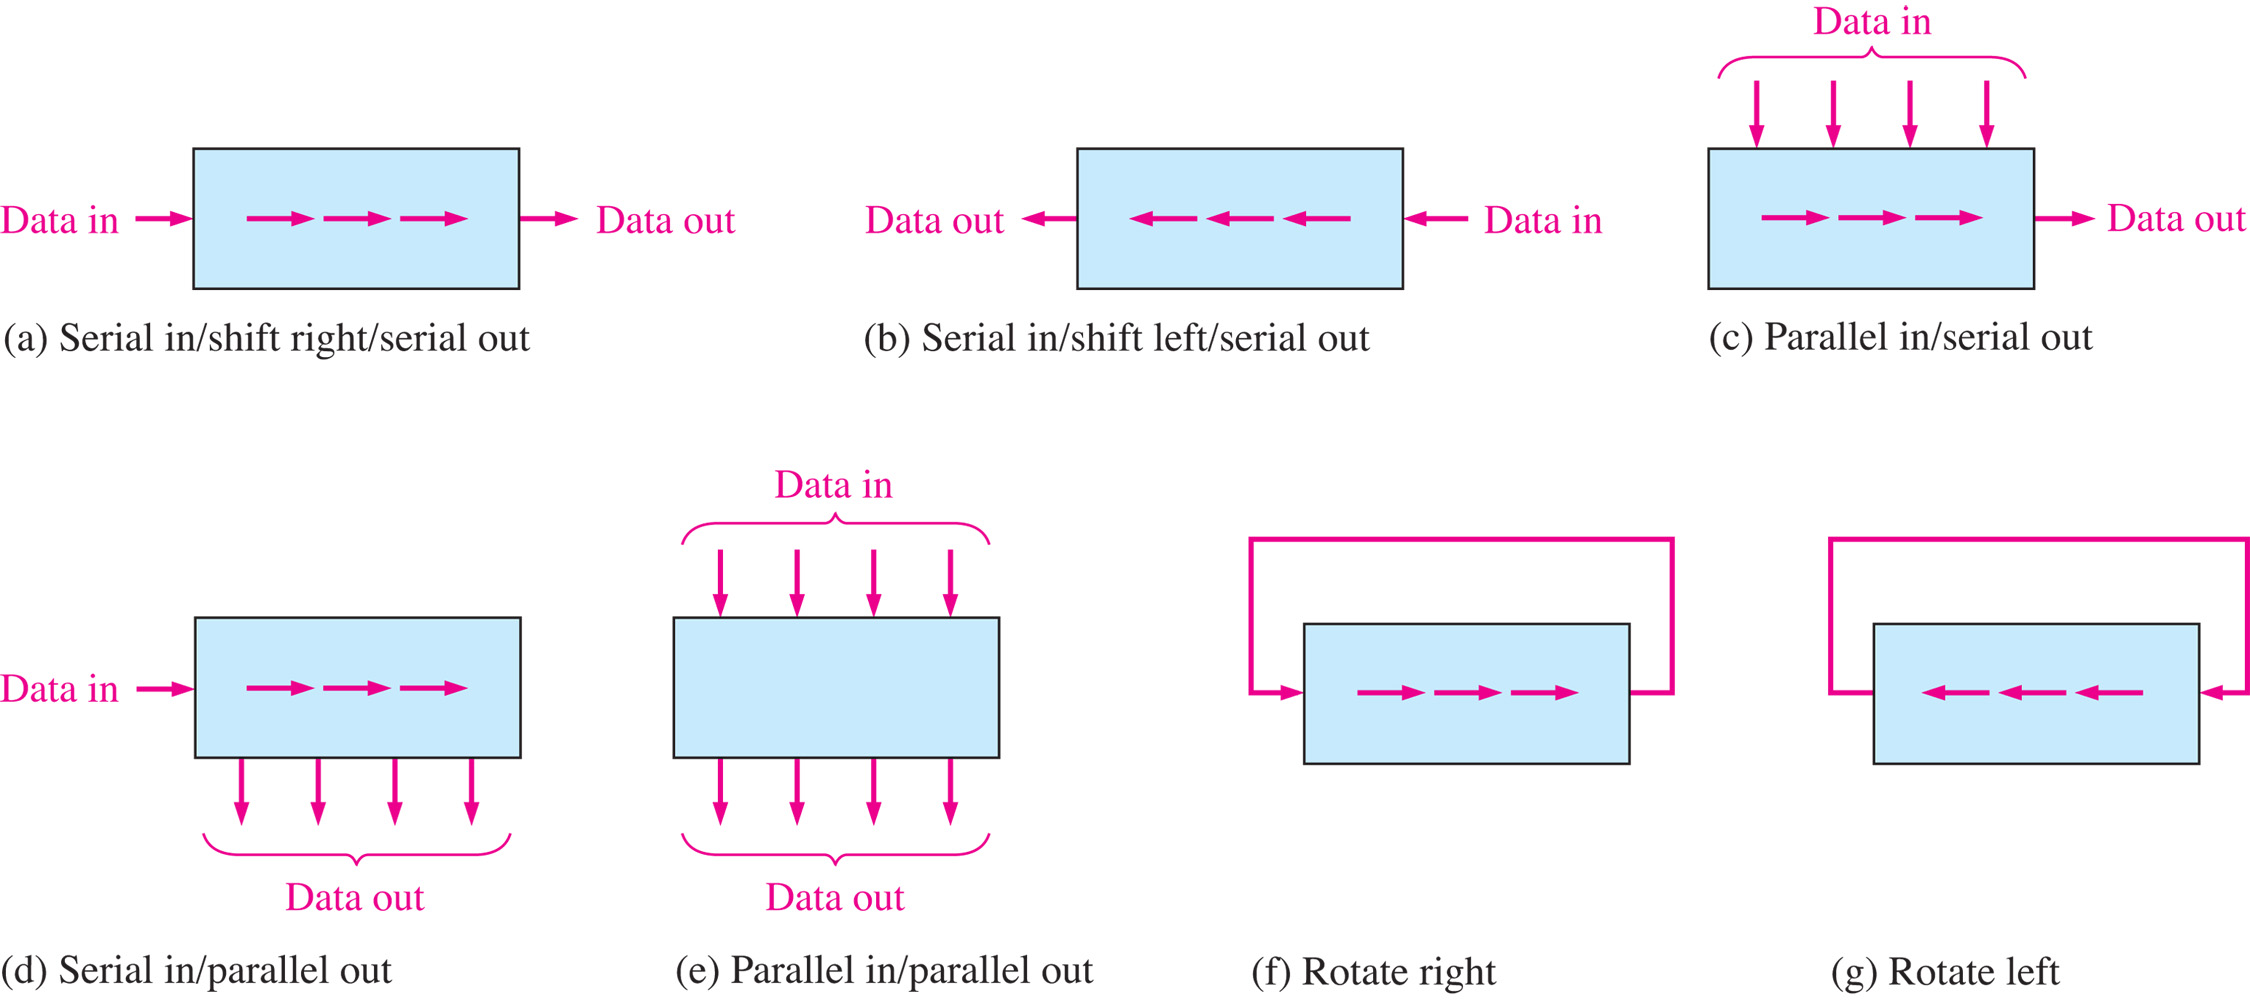
\includegraphics[width=0.6\textwidth]{figures/shift_1.jpg} \\ \vspace{0.2cm}
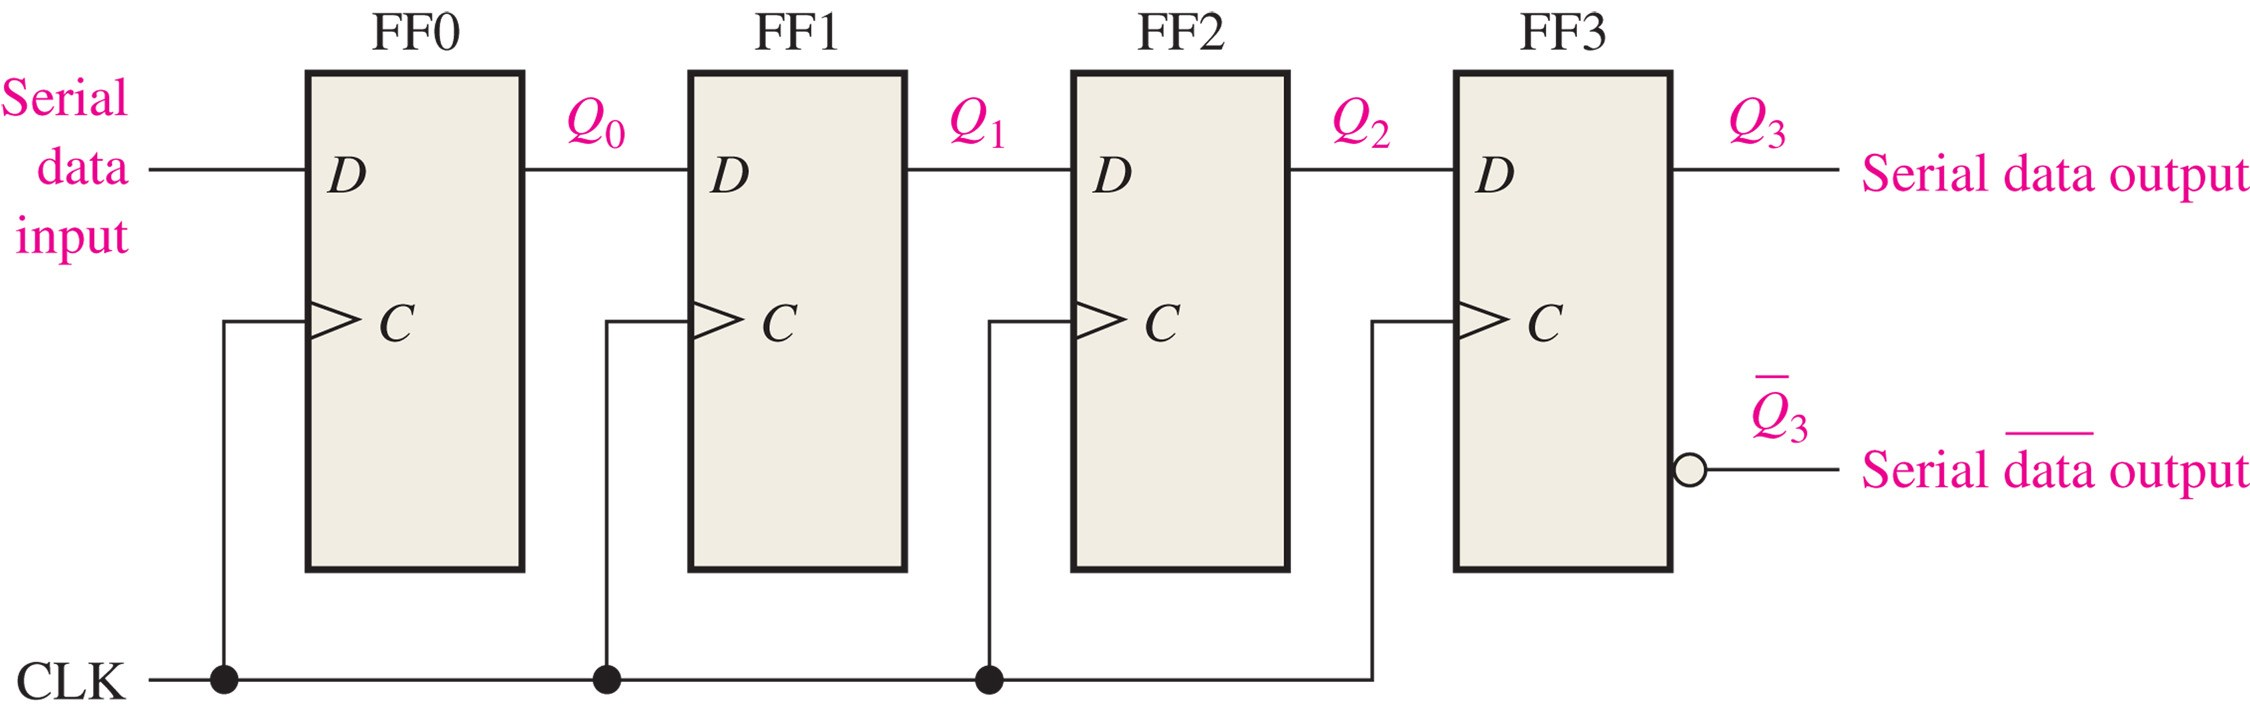
\includegraphics[width=0.6\textwidth]{figures/shift_4.jpg}
\caption{\small Different forms of shift register I/O.  Data in/out can be serial or parallel, and leftward or rightward.  Registers can be circular, rotating data.}
\end{figure}
\end{frame}

\begin{frame}{Shift register functions: load/shift}
\begin{figure}
\centering
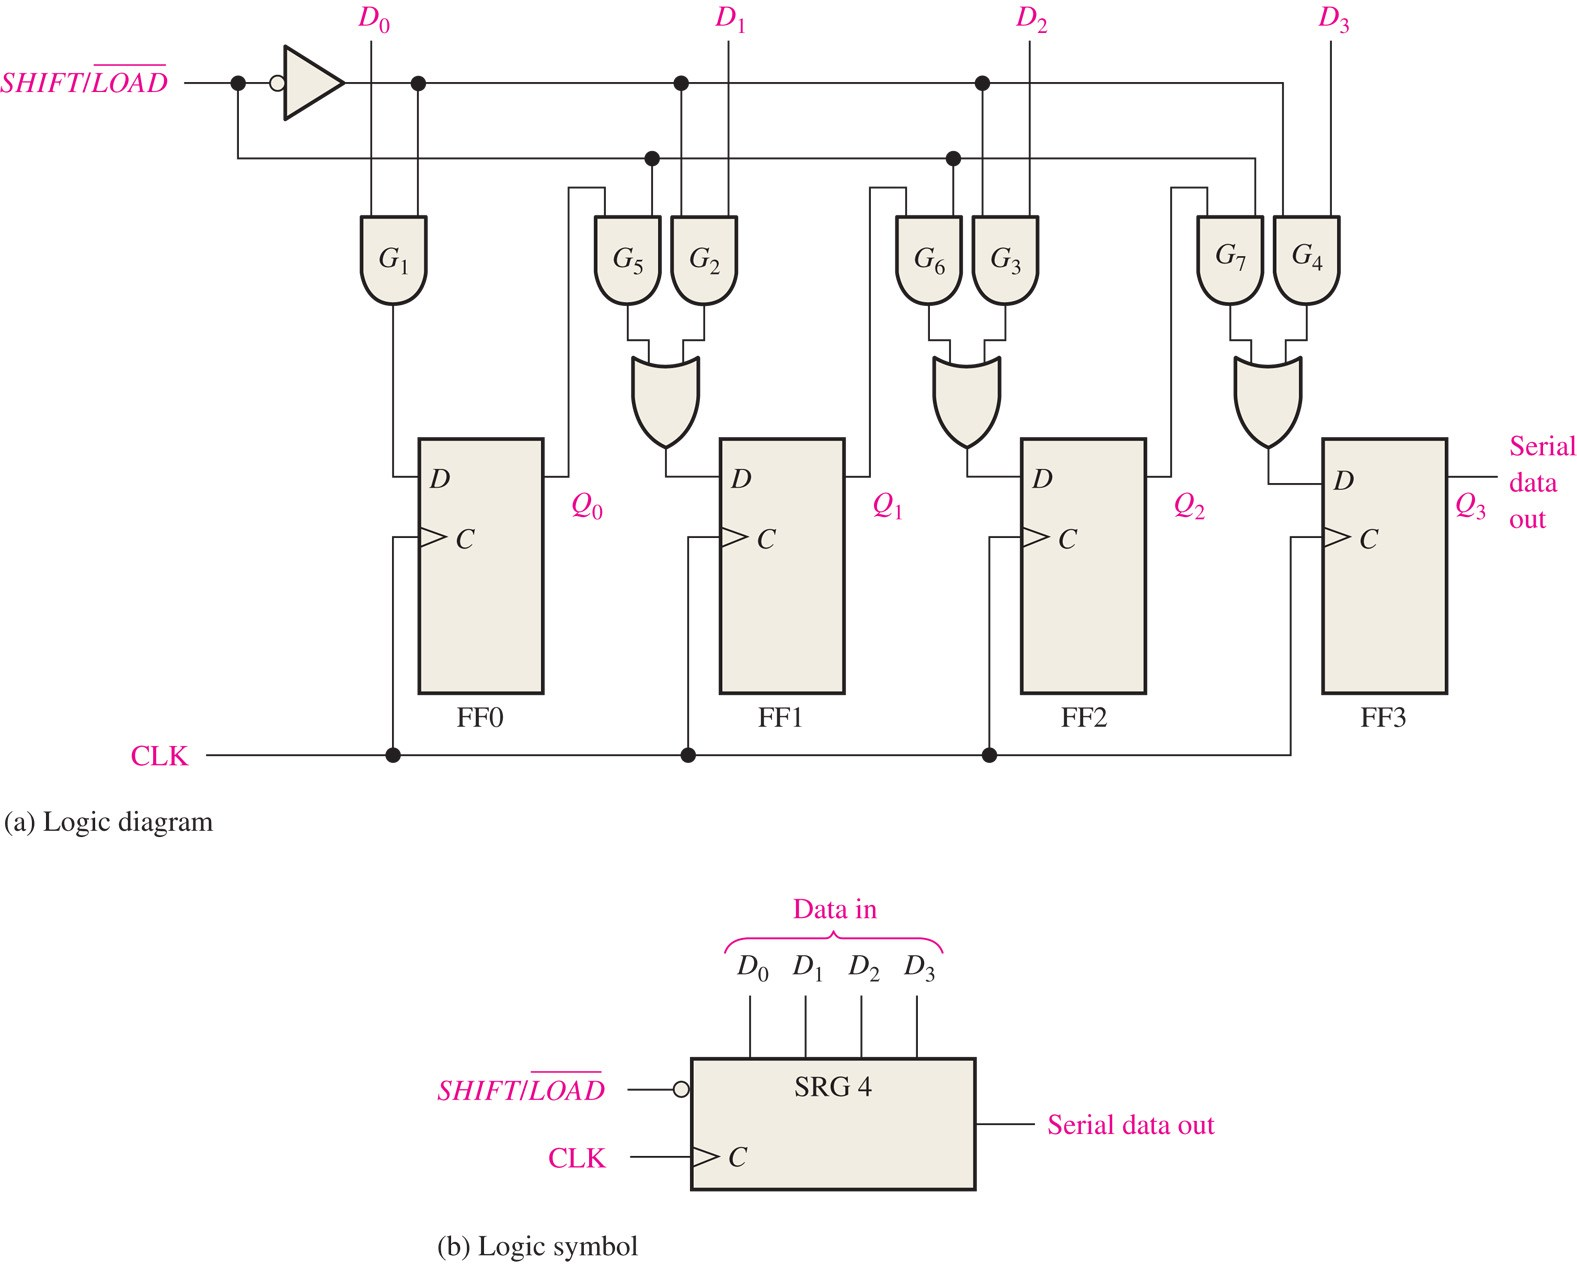
\includegraphics[width=0.7\textwidth]{figures/shift_2.jpg}
\caption{\small A 4-bit shift register from D flip-flops, with shift/load function.}
\end{figure}
\end{frame}

\begin{frame}{Shift register functions: load/shift}
\begin{figure}
\centering
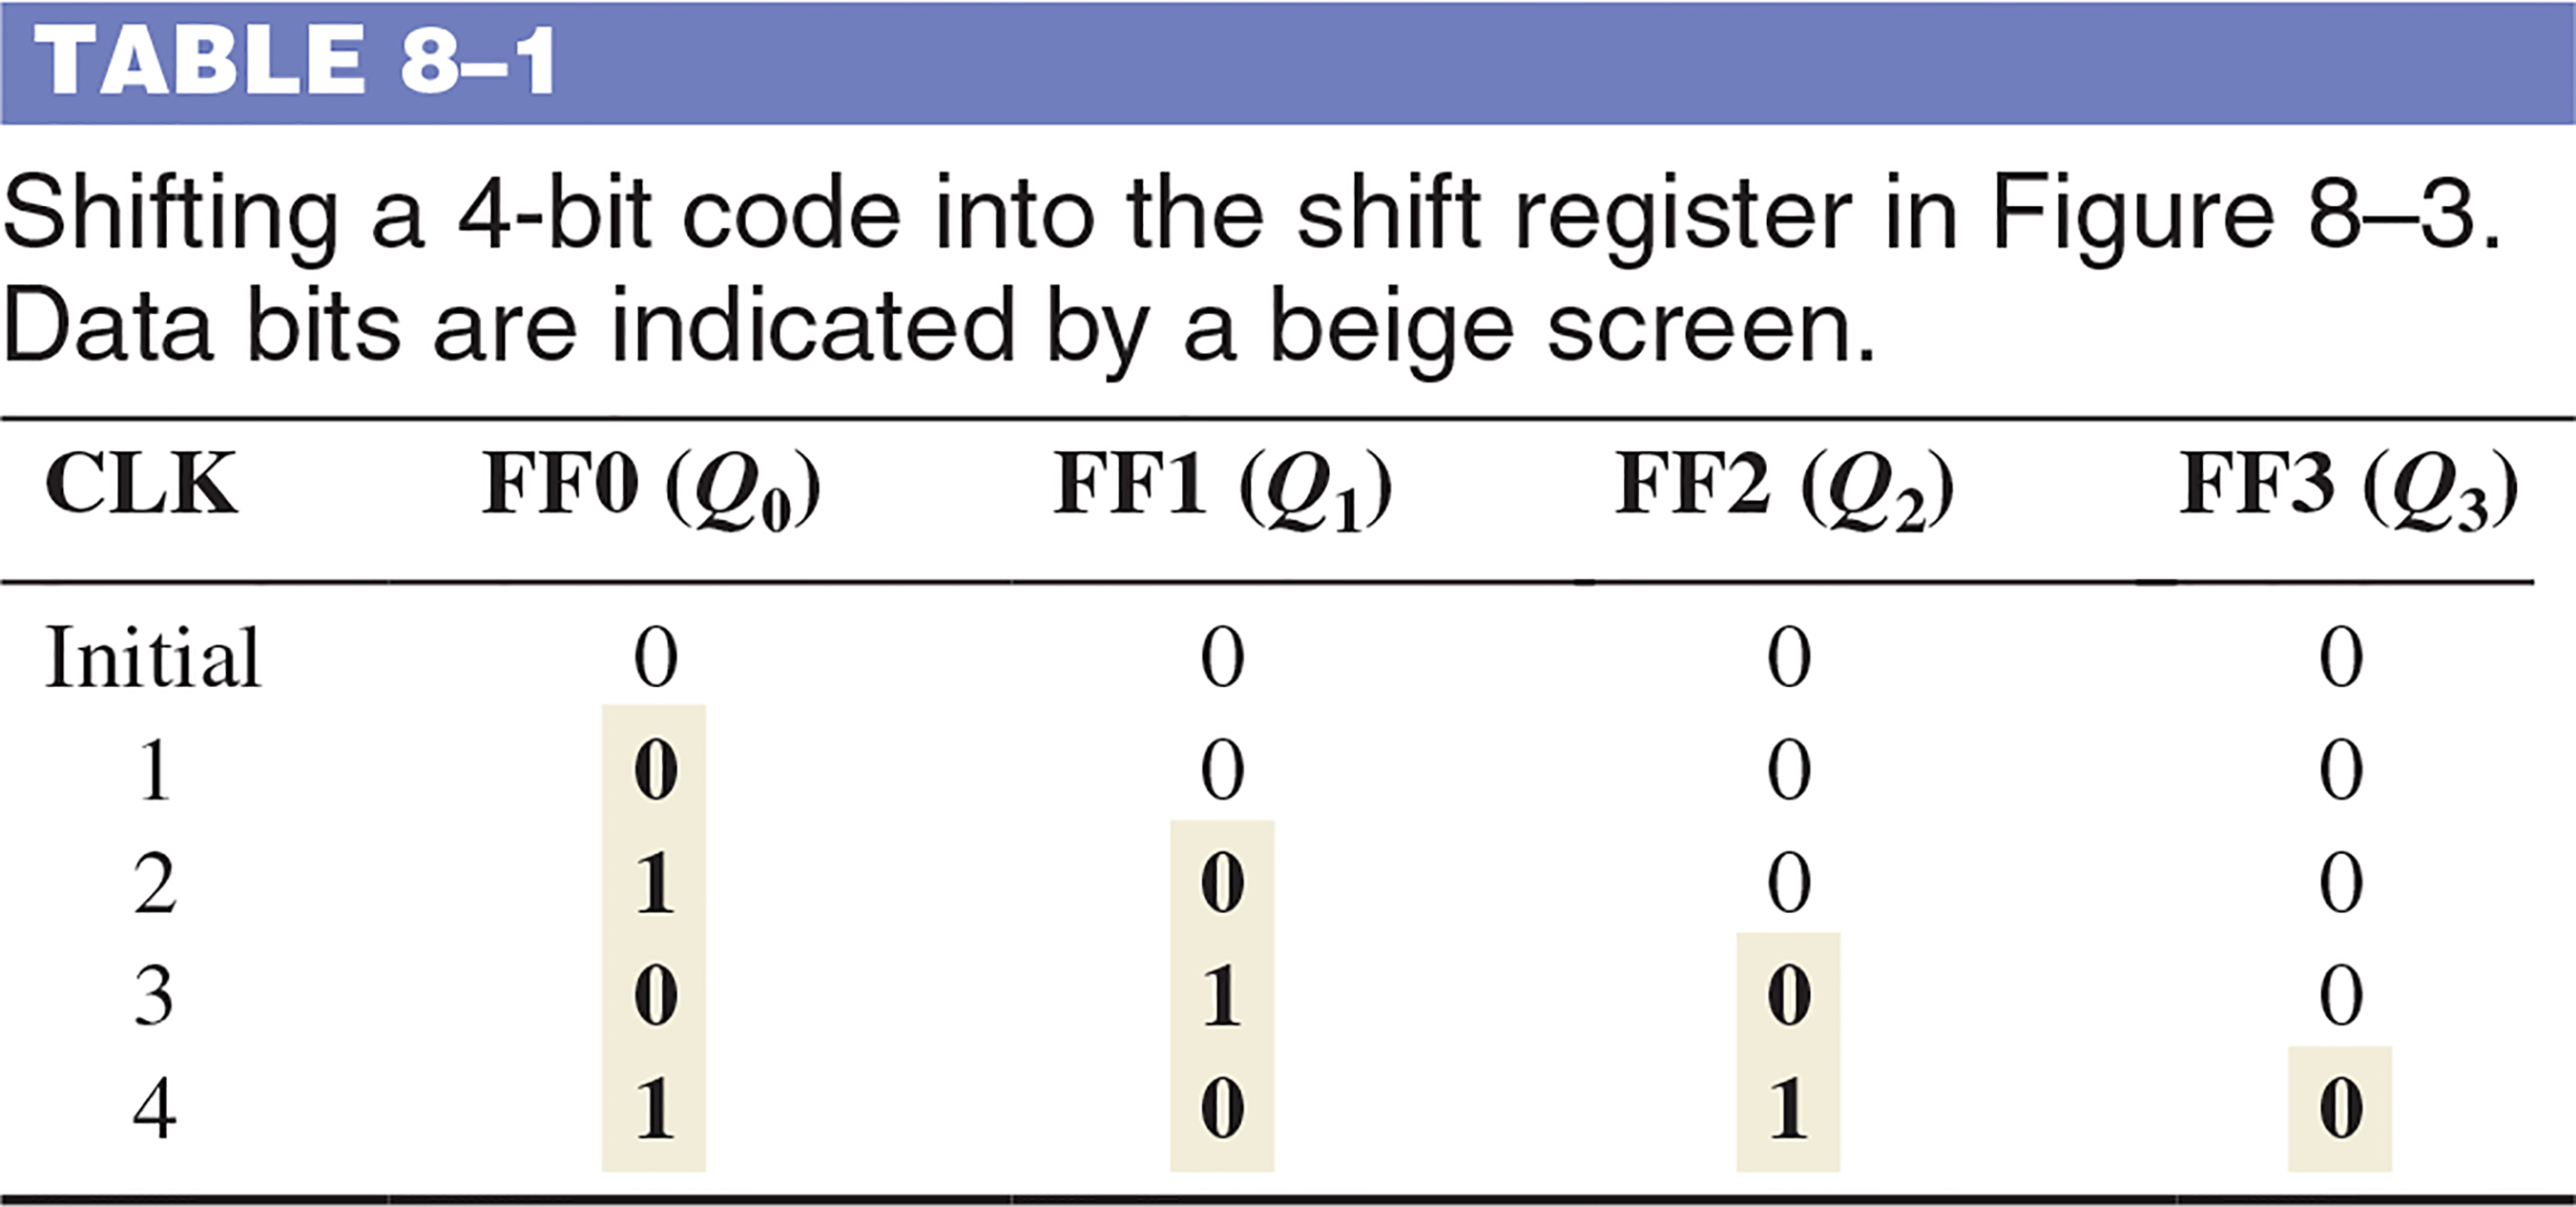
\includegraphics[width=0.45\textwidth]{figures/shift_5.jpg}
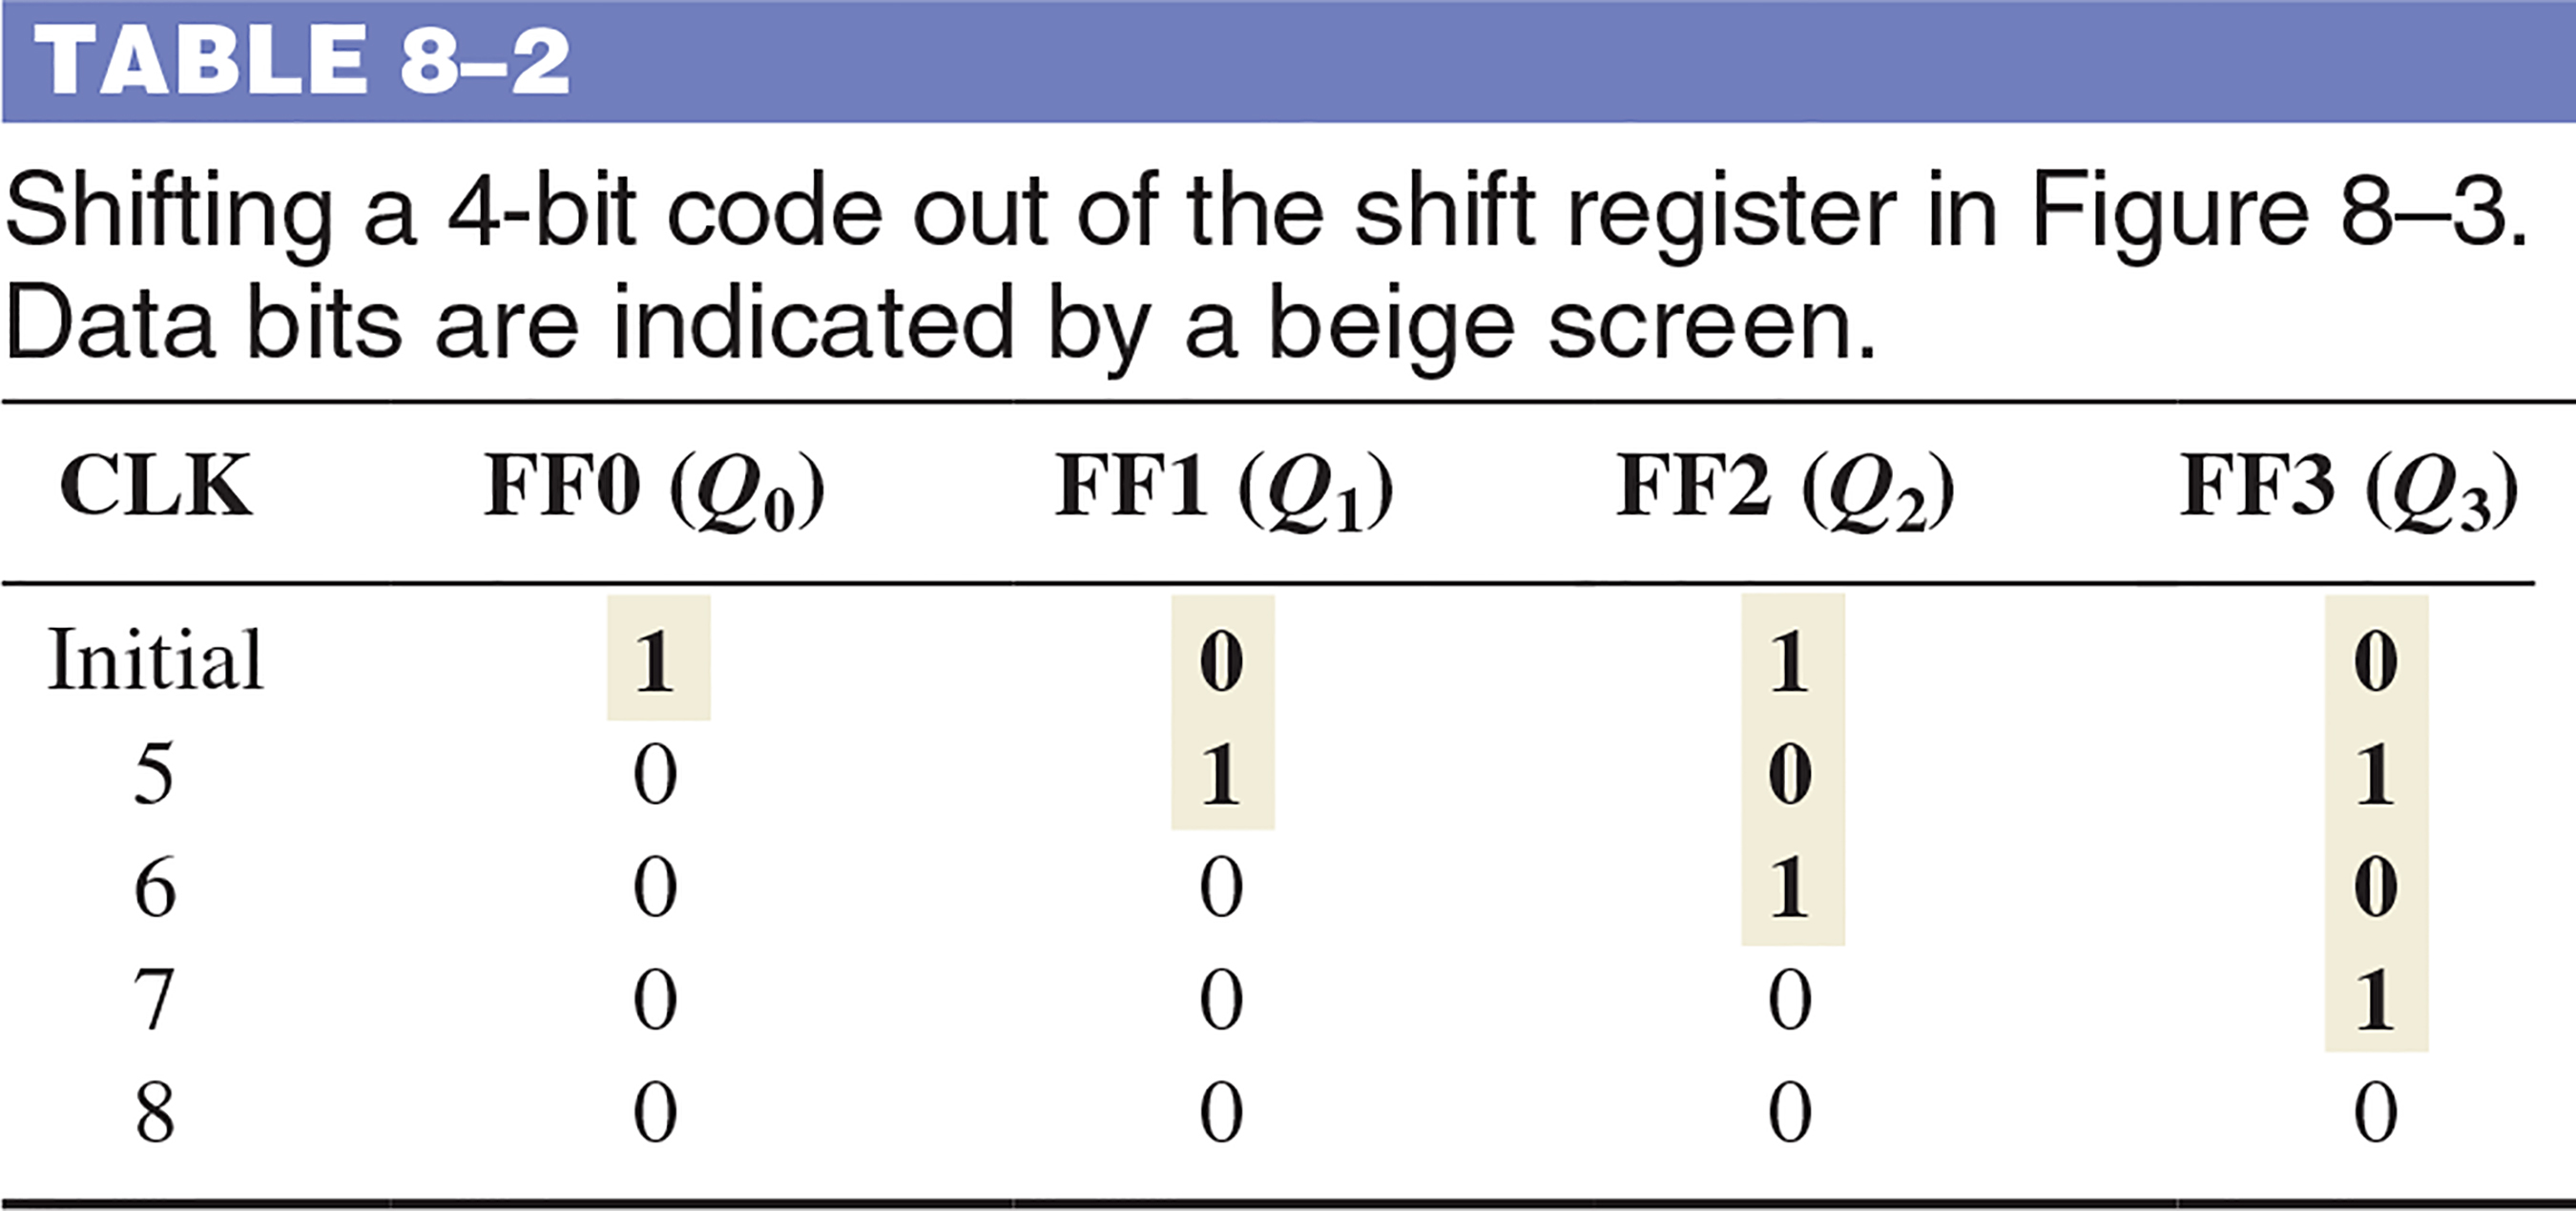
\includegraphics[width=0.45\textwidth]{figures/shift_6.jpg}
\caption{\small Shifting a 4-bit sequence into a 4-bit shift-register.}
\end{figure}
\begin{itemize}
\item Note the direction of data flow.
\item Data bits are initially RESET.
\item Positive edge CLK pulses advance data.
\end{itemize}
\end{frame}

\begin{frame}{Shift register functions: bidirectional}
\begin{figure}
\centering
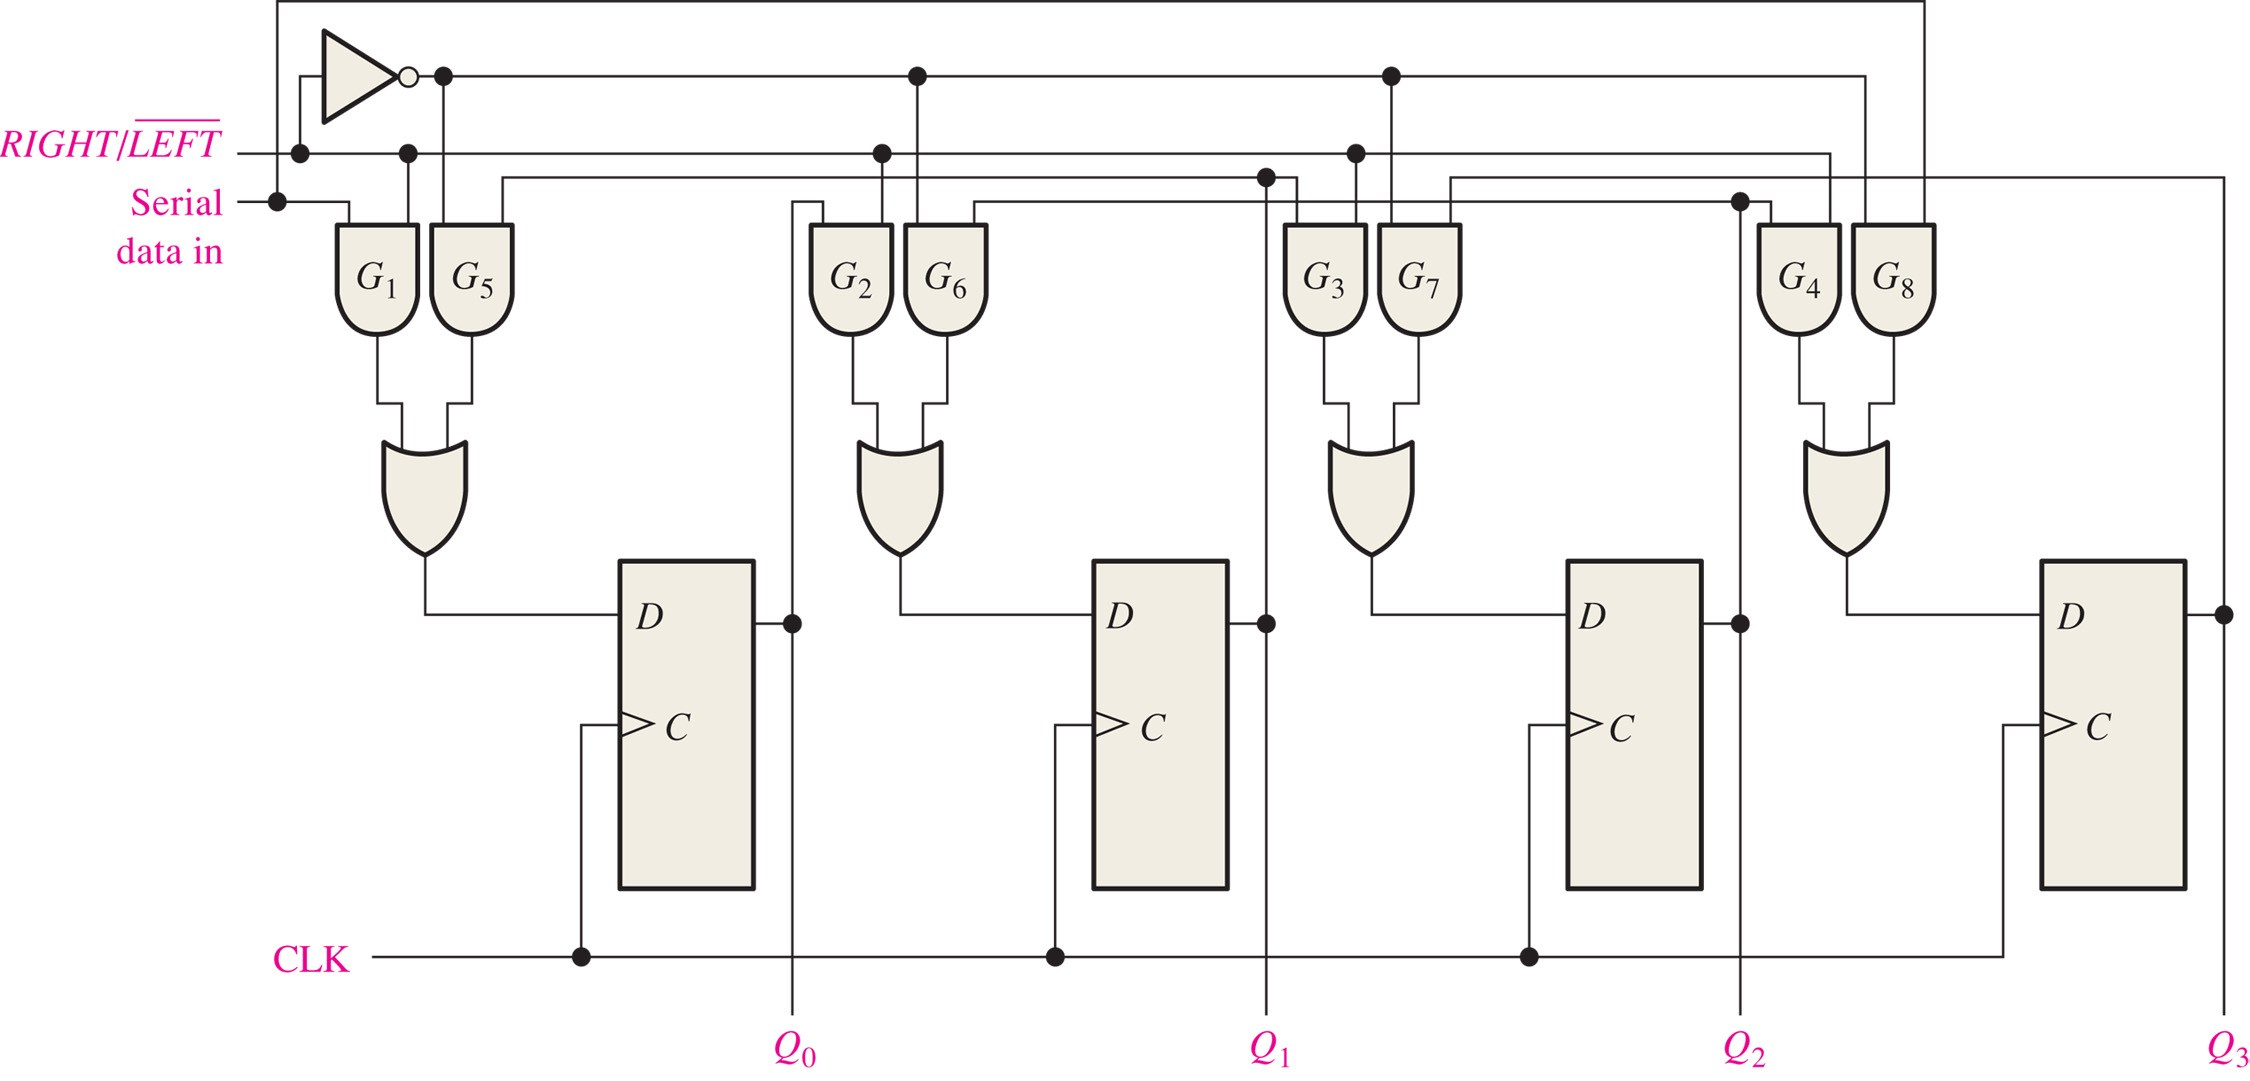
\includegraphics[width=0.8\textwidth]{figures/shift_8.jpg}
\caption{\small A 4-bit shift register from D flip-flops, with bidirectional function.}
\end{figure}
\begin{itemize}
\item Note \textit{backward connections.}
\item Steering gates load rightward or leftward data.
\end{itemize}
\end{frame}

\begin{frame}{Shift register functions: bidirectional}
\begin{figure}
\centering
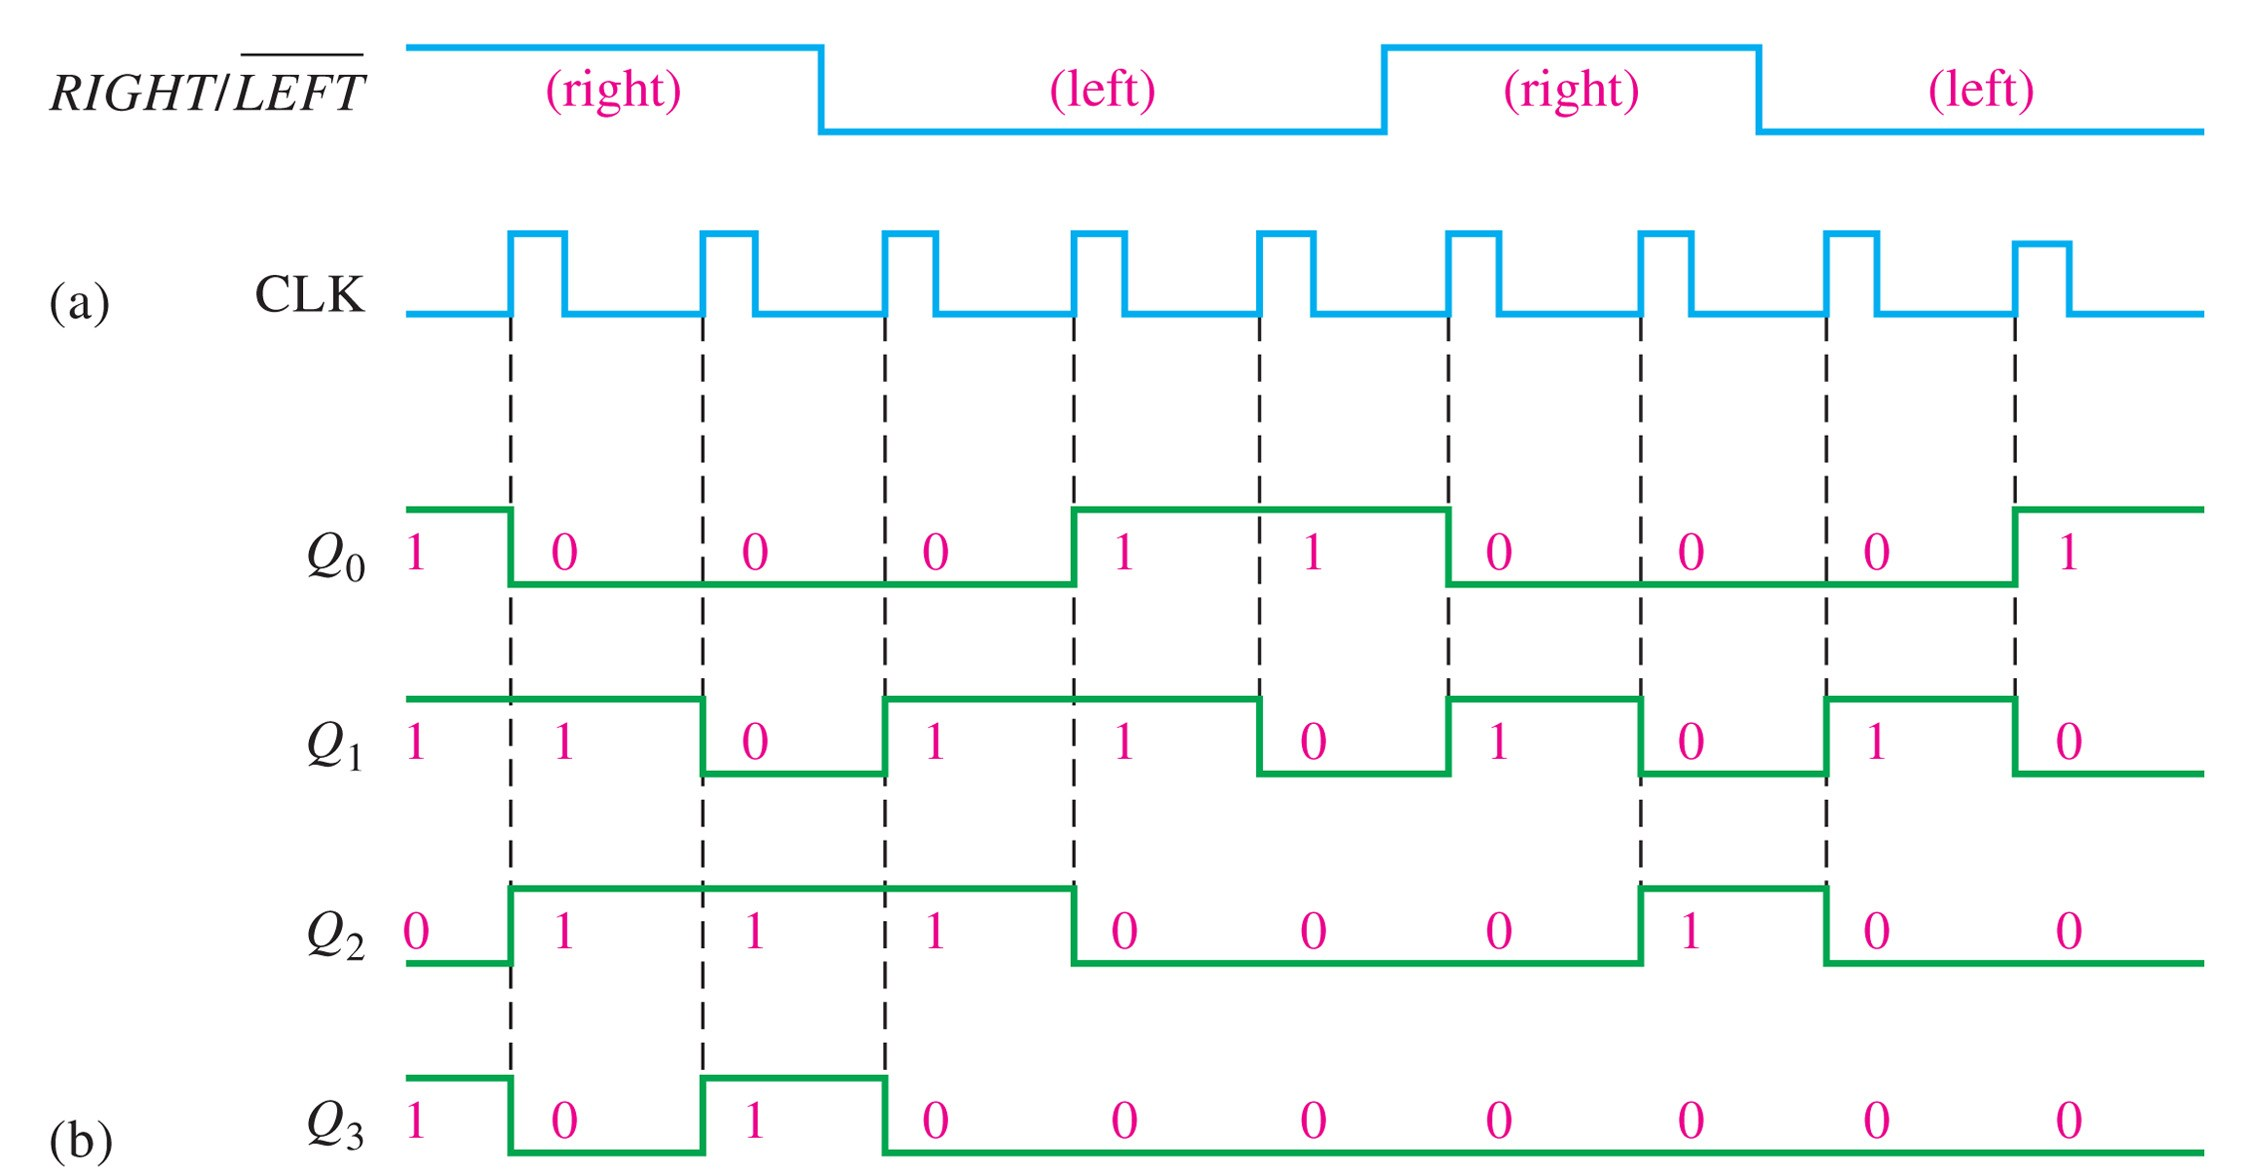
\includegraphics[width=0.8\textwidth]{figures/shift_9.jpg}
\caption{\small A 4-bit shift register from D flip-flops, with bidirectional function.}
\end{figure}
\begin{itemize}
\item Note \textit{backward connections.}
\item Steering gates load rightward or leftward data.
\end{itemize}
\end{frame}

\begin{frame}{Shift register counters: Johnson counters}
\begin{figure}
\centering
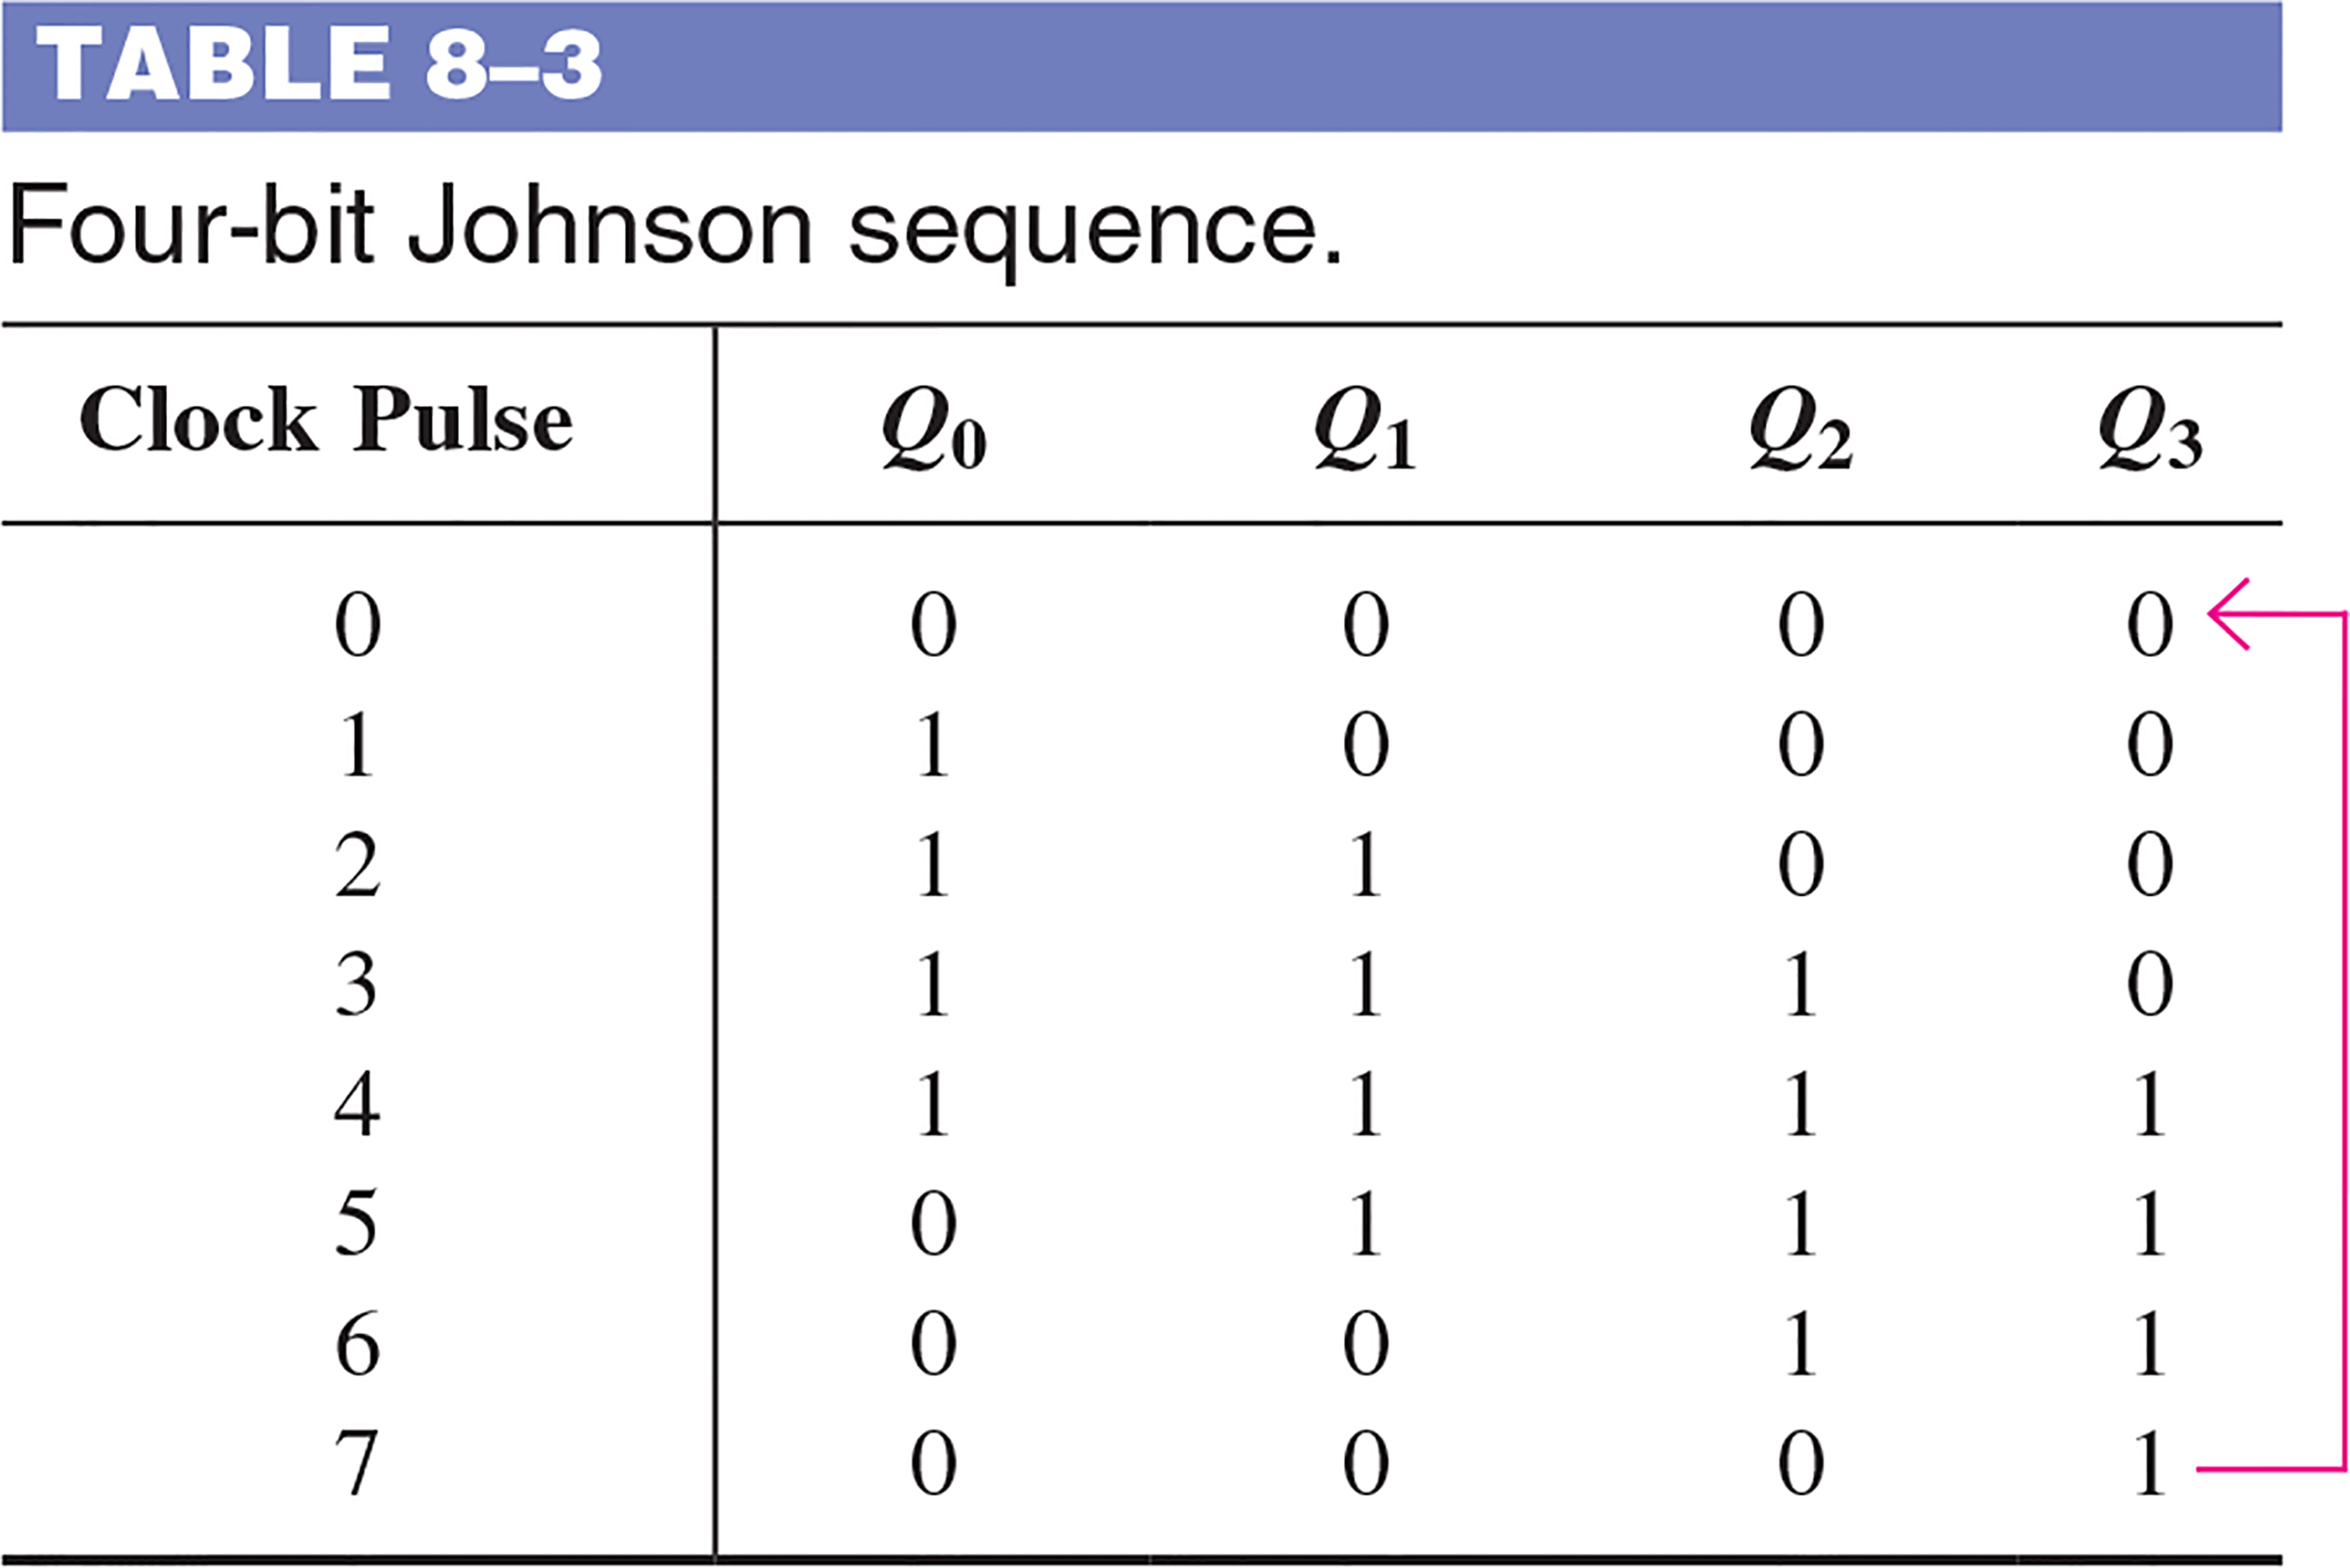
\includegraphics[width=0.45\textwidth]{figures/shift_10.jpg} \hspace{0.25cm}
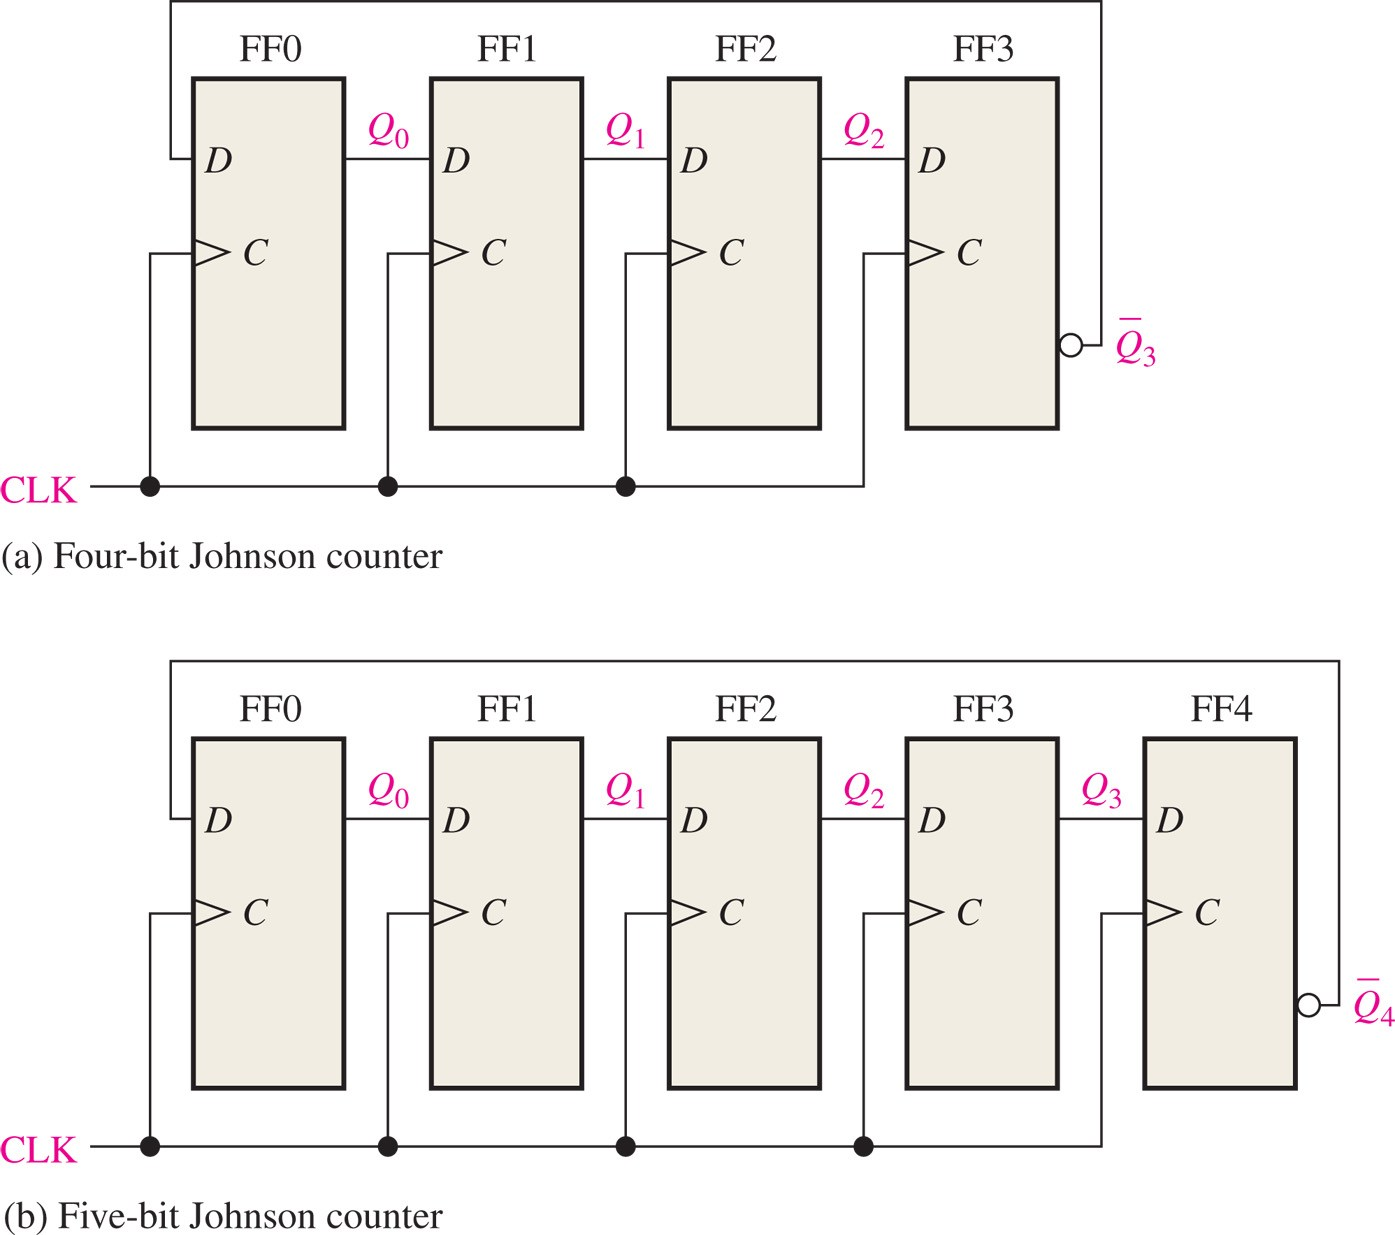
\includegraphics[width=0.45\textwidth]{figures/shift_11.jpg}
\caption{\small (Left) A 4-bit Johnson counter state sequence. (Right) Circuit diagram of Johnson counters.}
\end{figure}
\begin{itemize}
\item Note the output requires a decoder.
\item Final output is active LOW.
\end{itemize}
\end{frame}

\begin{frame}{Shift register counters: ring counters}
\begin{figure}
\centering
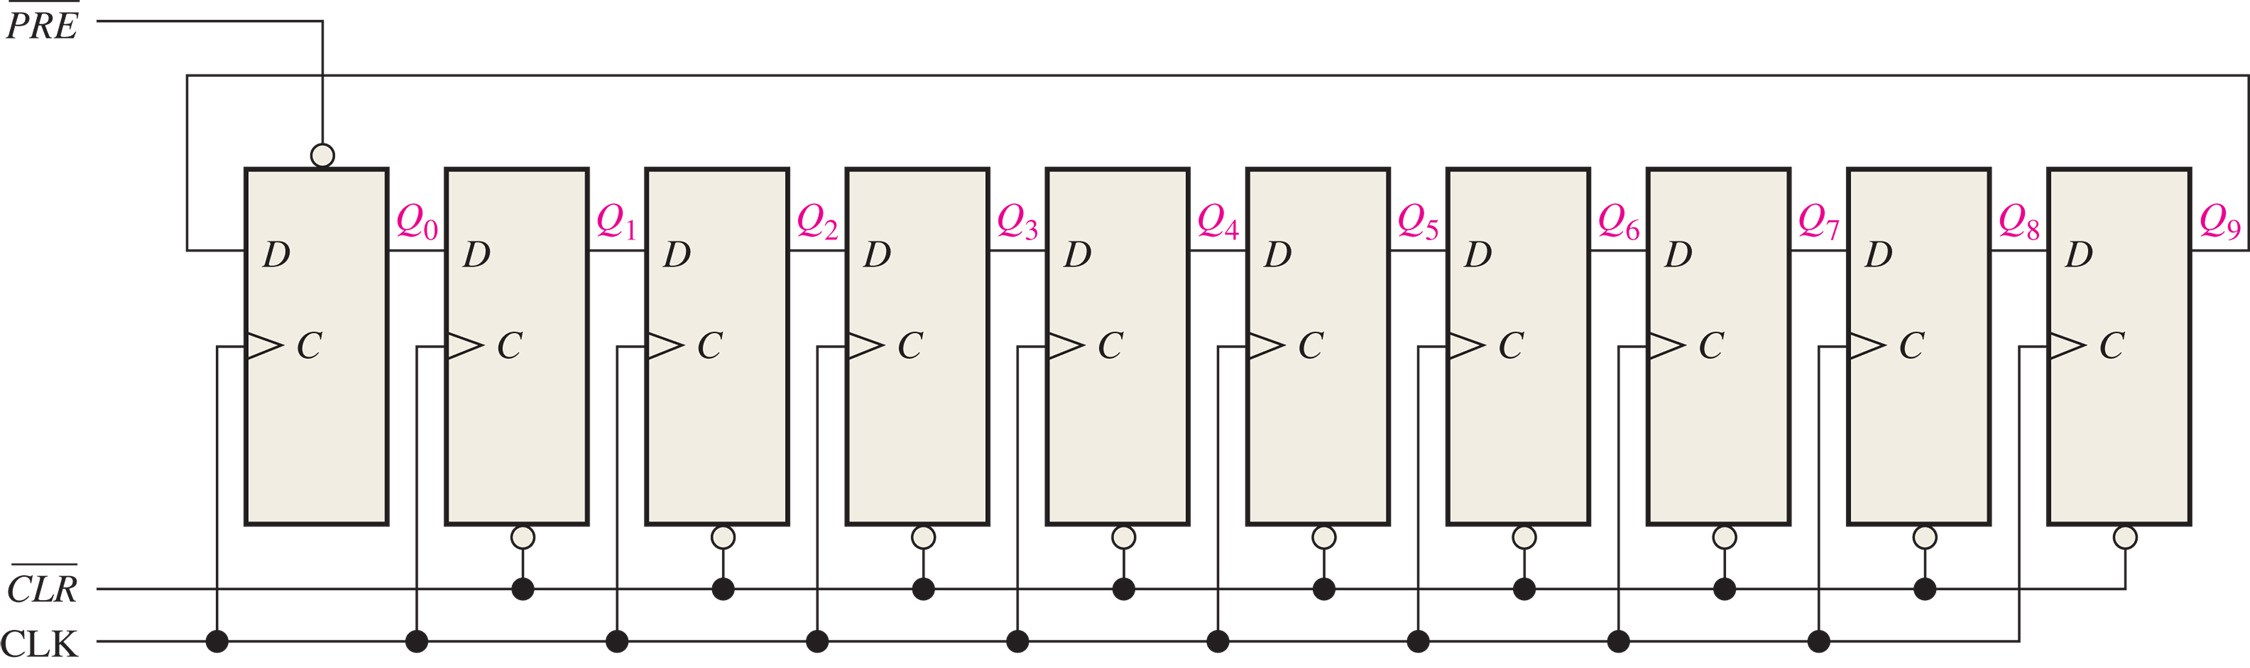
\includegraphics[width=0.65\textwidth]{figures/shift_12.jpg} \\ \vspace{0.5cm}
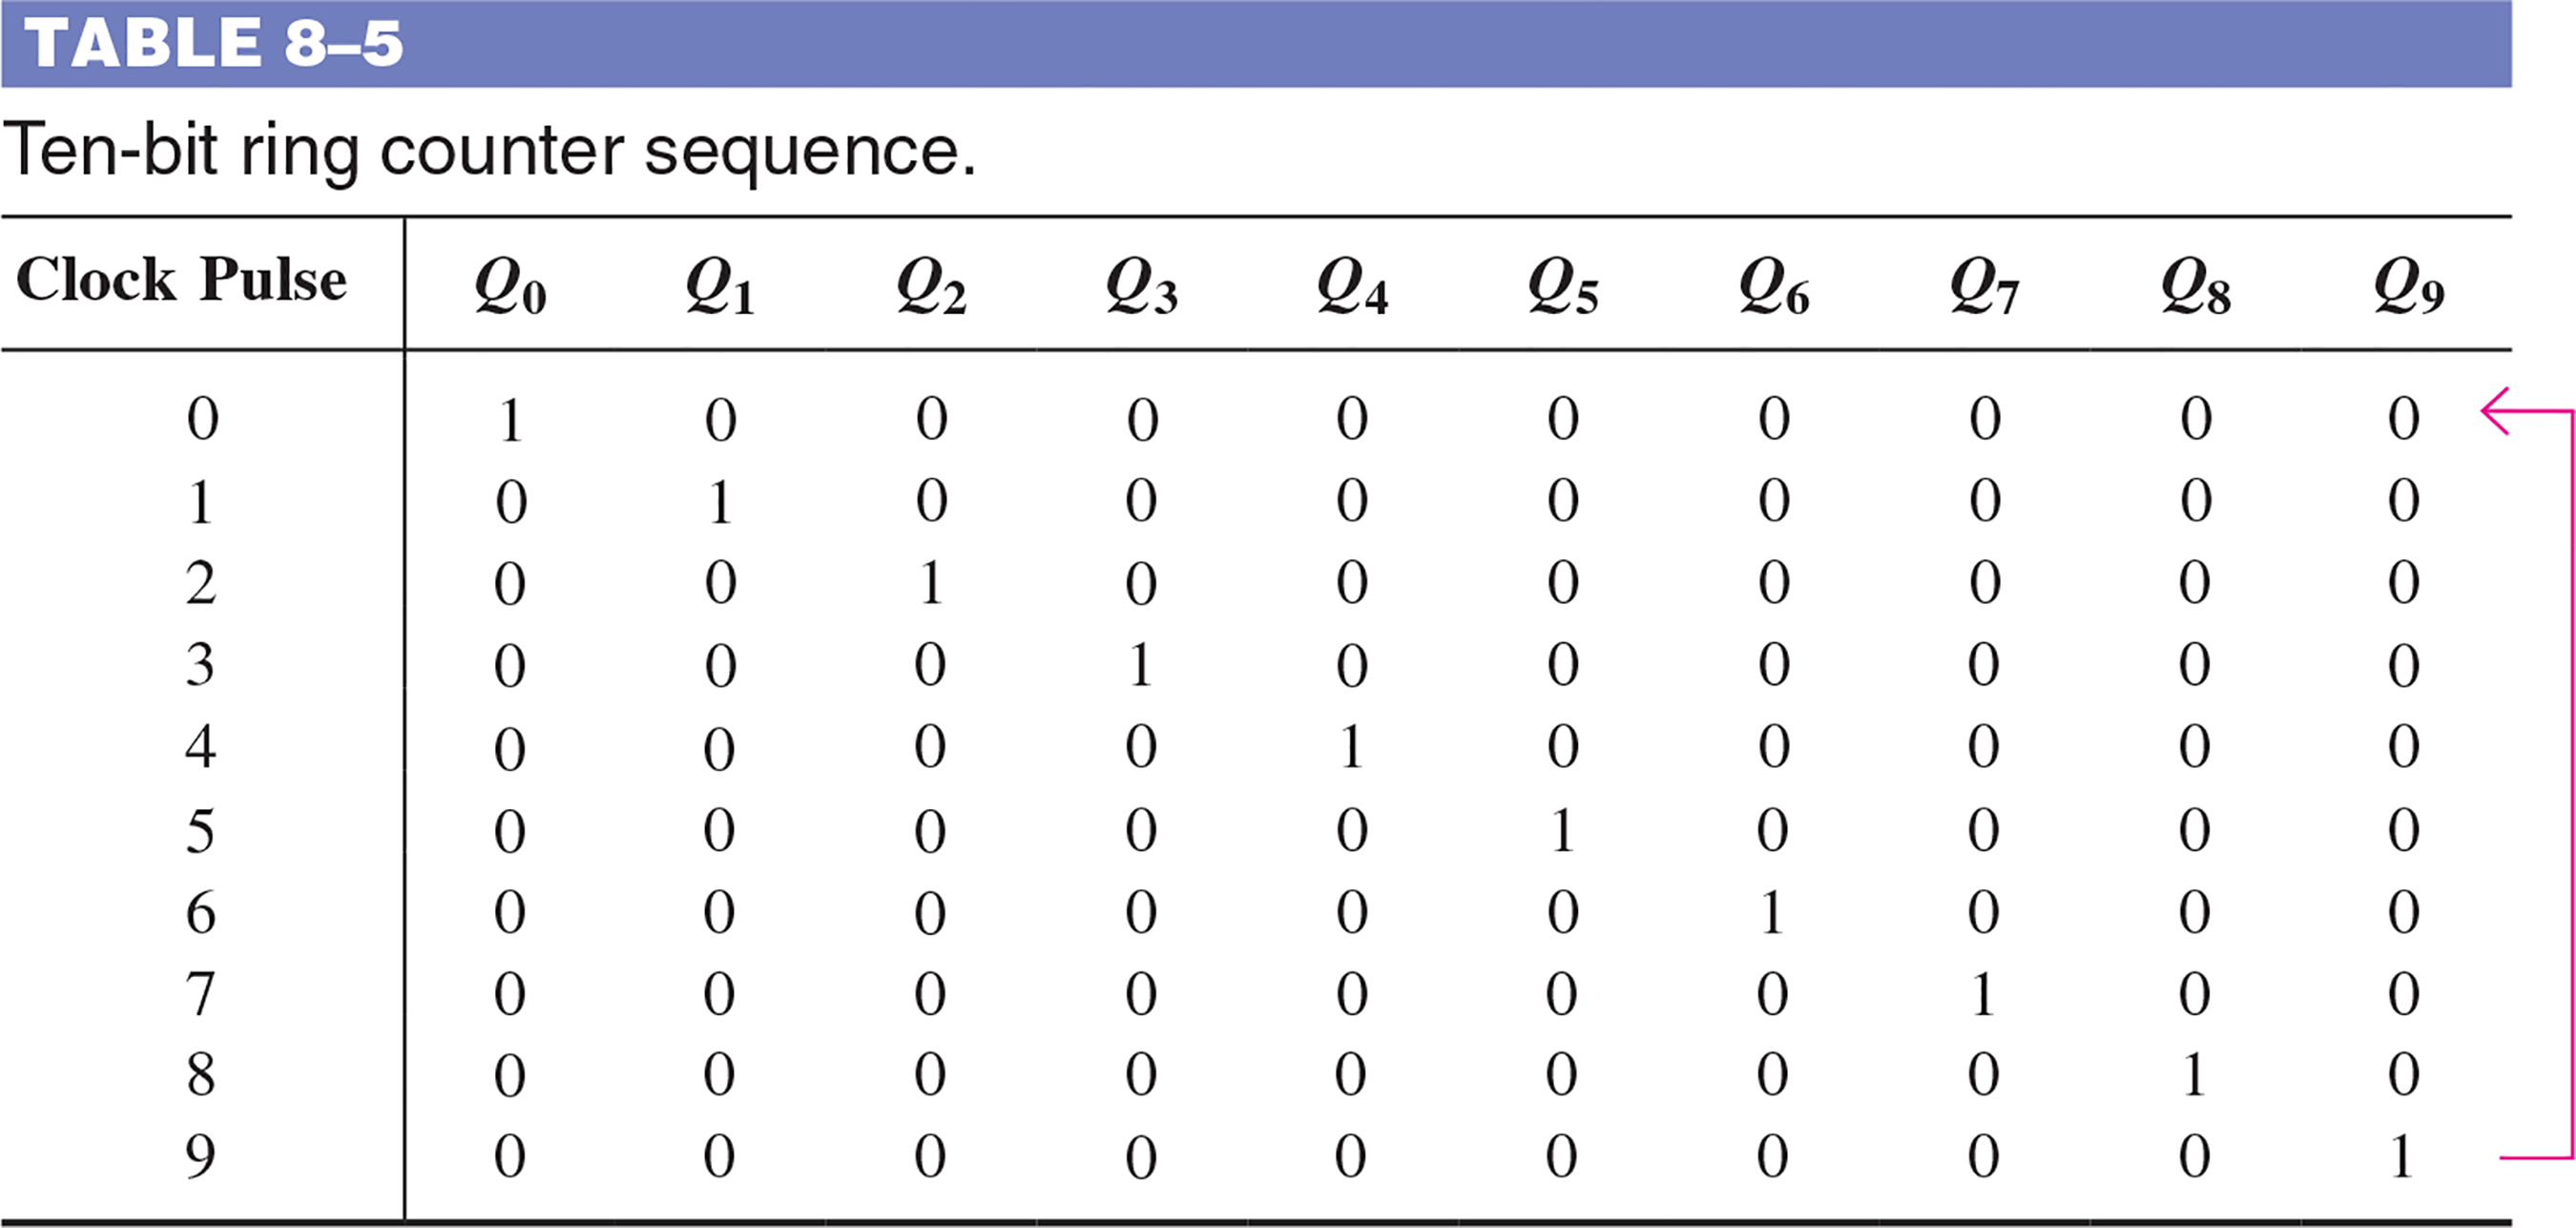
\includegraphics[width=0.55\textwidth]{figures/shift_13.jpg}
\caption{\small (Top) A 10-bit ring counter diagram. (Bottom) States corresponing to the ring counter. Note the output requires a decoder.}
\end{figure}
\end{frame}

\begin{frame}{Shift register applications: time-delay}
\begin{figure}
\centering
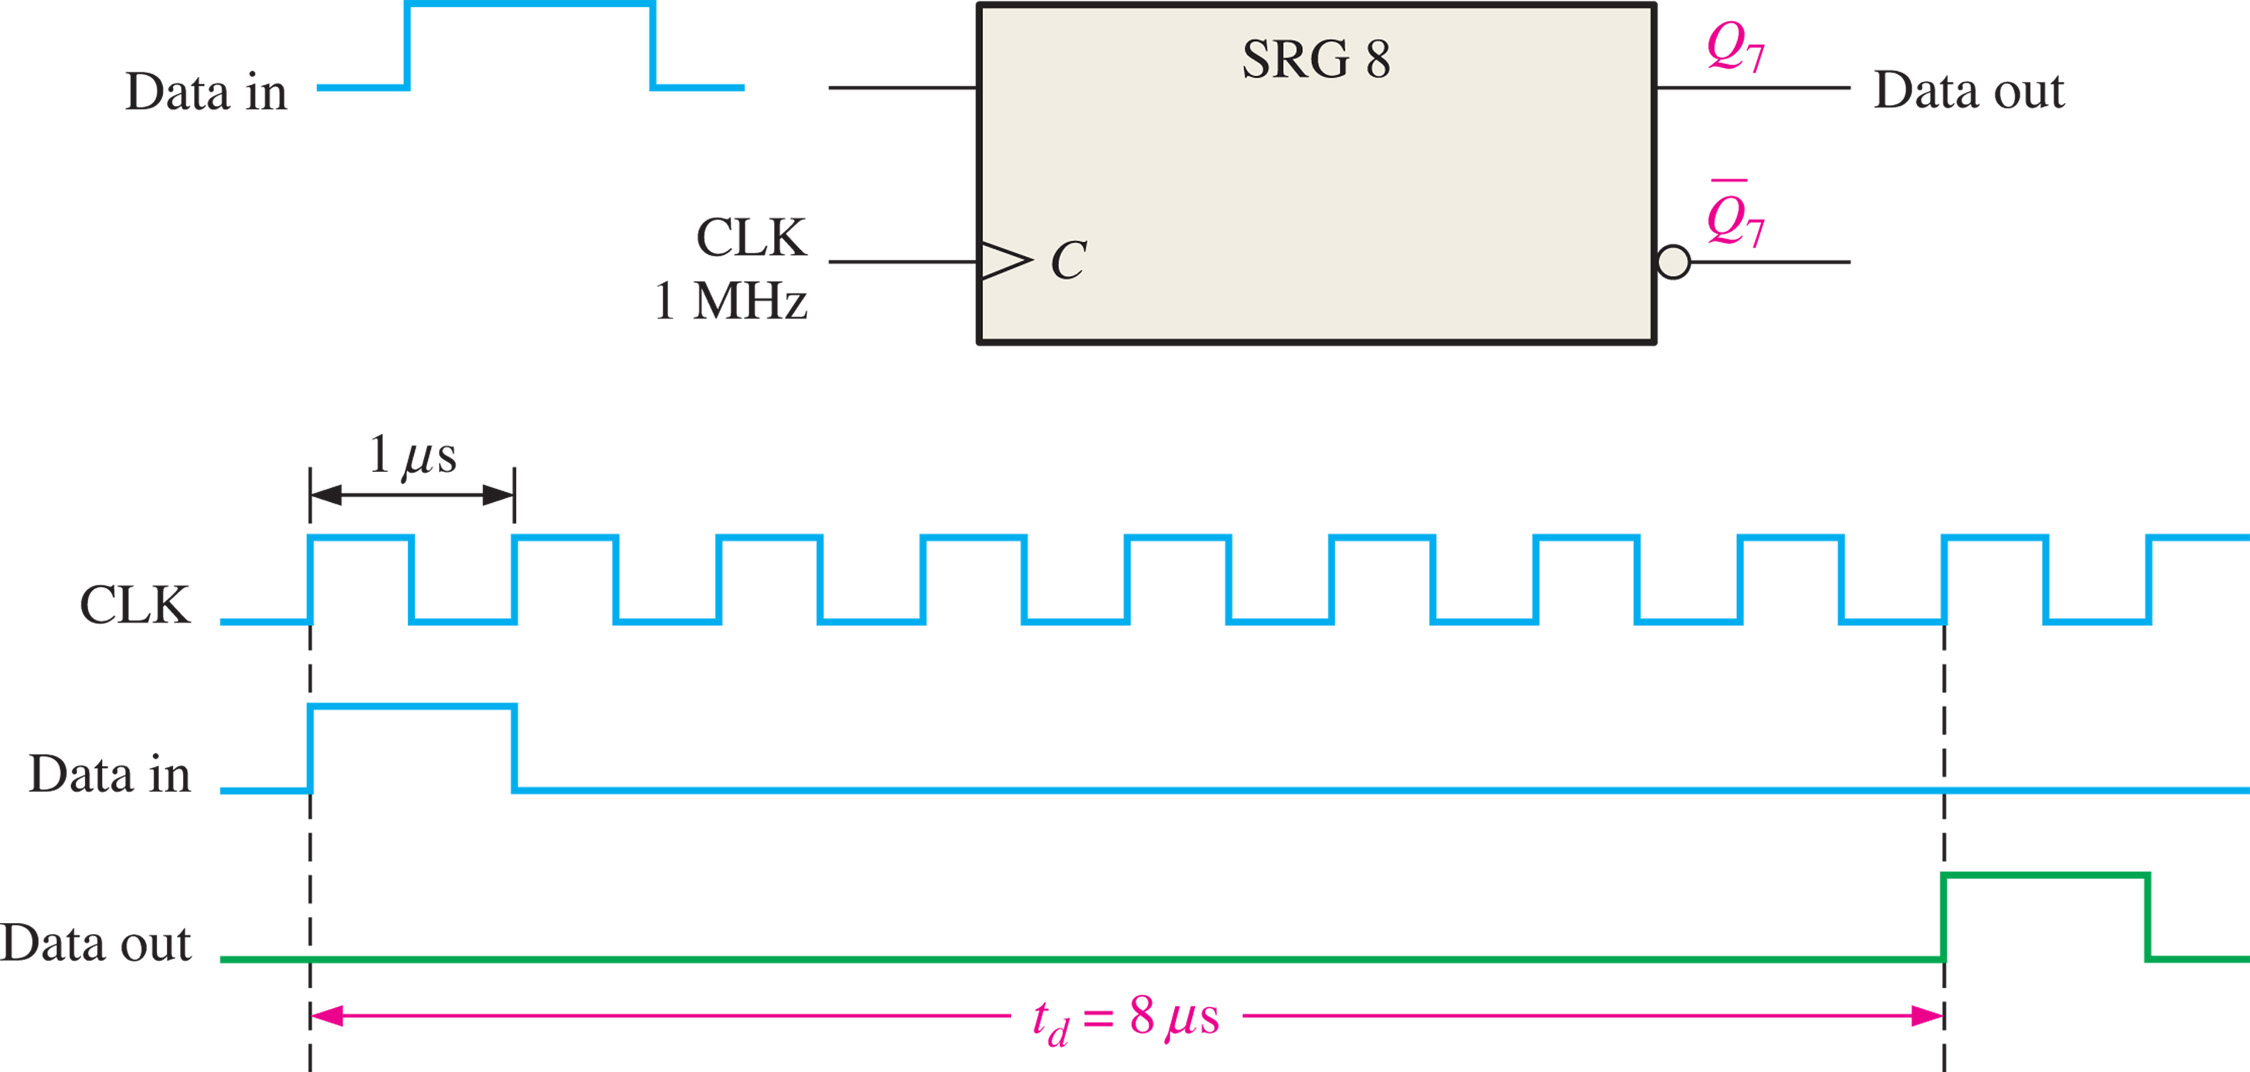
\includegraphics[width=0.65\textwidth]{figures/shift_14.jpg}
\caption{\small (Top) An 8-bit shift register as a time-delay. (Bottom) Corresponding timing diagram assuming 1 MHz CLK frequency.}
\end{figure}
\end{frame}

\begin{frame}{Shift register applications: serial to parallel data conversion}
\begin{figure}
\centering
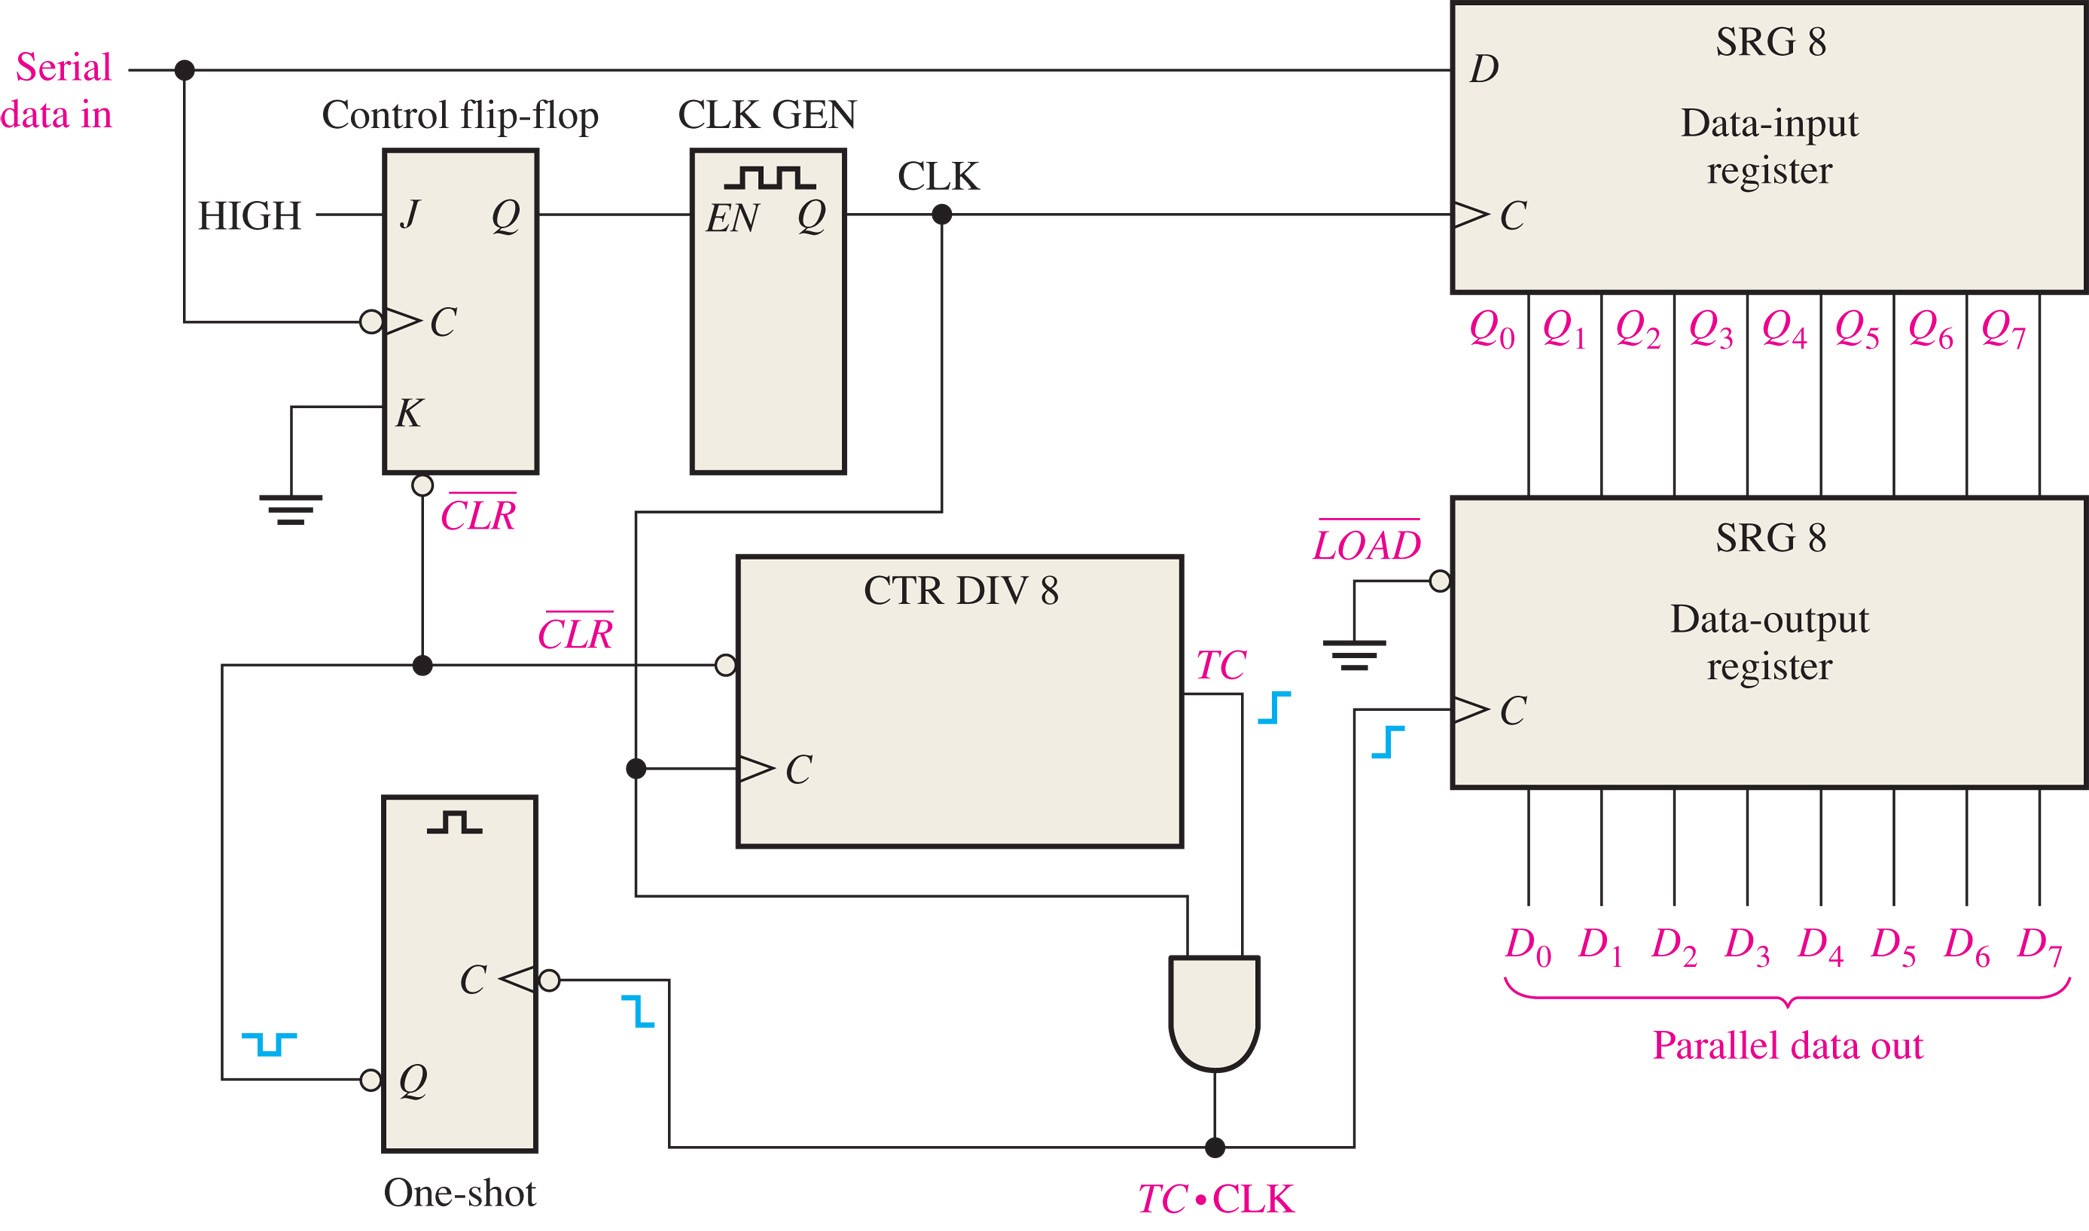
\includegraphics[width=0.75\textwidth]{figures/shift_15.jpg} \\ \vspace{0.5cm}
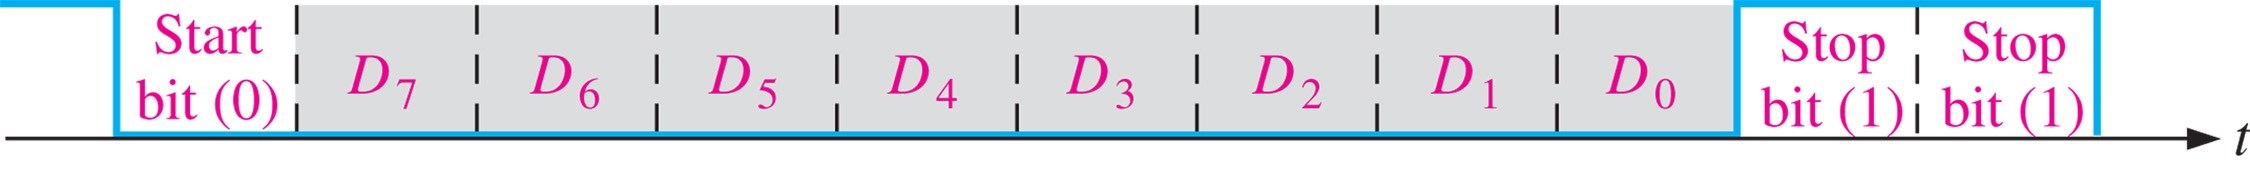
\includegraphics[width=0.75\textwidth]{figures/shift_16.jpg}
\caption{\small (Top) Serial to parallel data converter circuit diagram. (Bottom) Concept of start and stop bits.}
\end{figure}
\end{frame}

\begin{frame}{Shift register applications: serial to parallel data conversion}
\begin{figure}
\centering
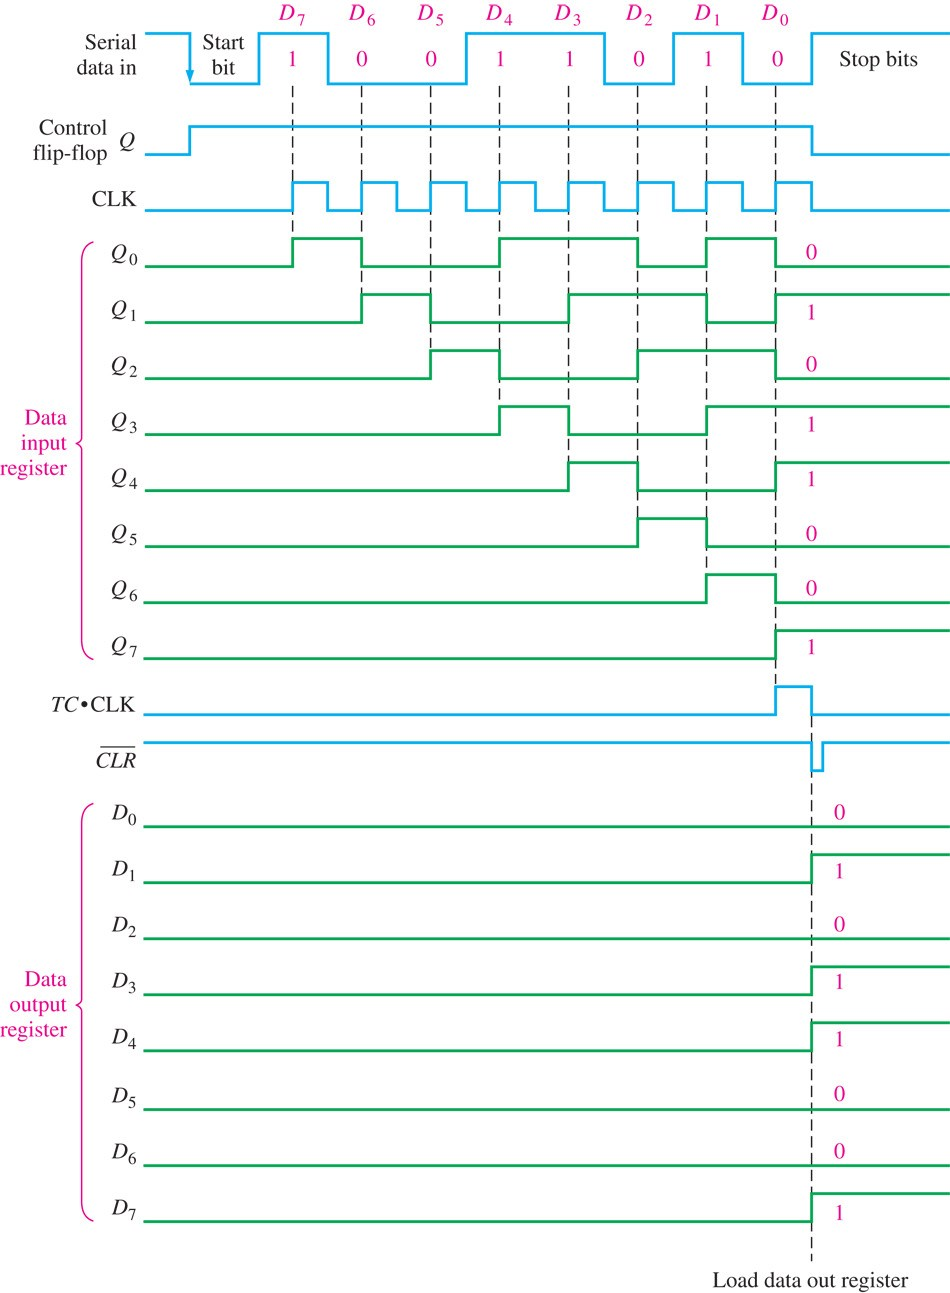
\includegraphics[width=0.45\textwidth]{figures/shift_17.jpg}
\caption{\small Timing diagram of the converter.}
\end{figure}
\end{frame}

\section{Counters}

\begin{frame}{Counters: Finite State Machines}
\begin{figure}
\centering
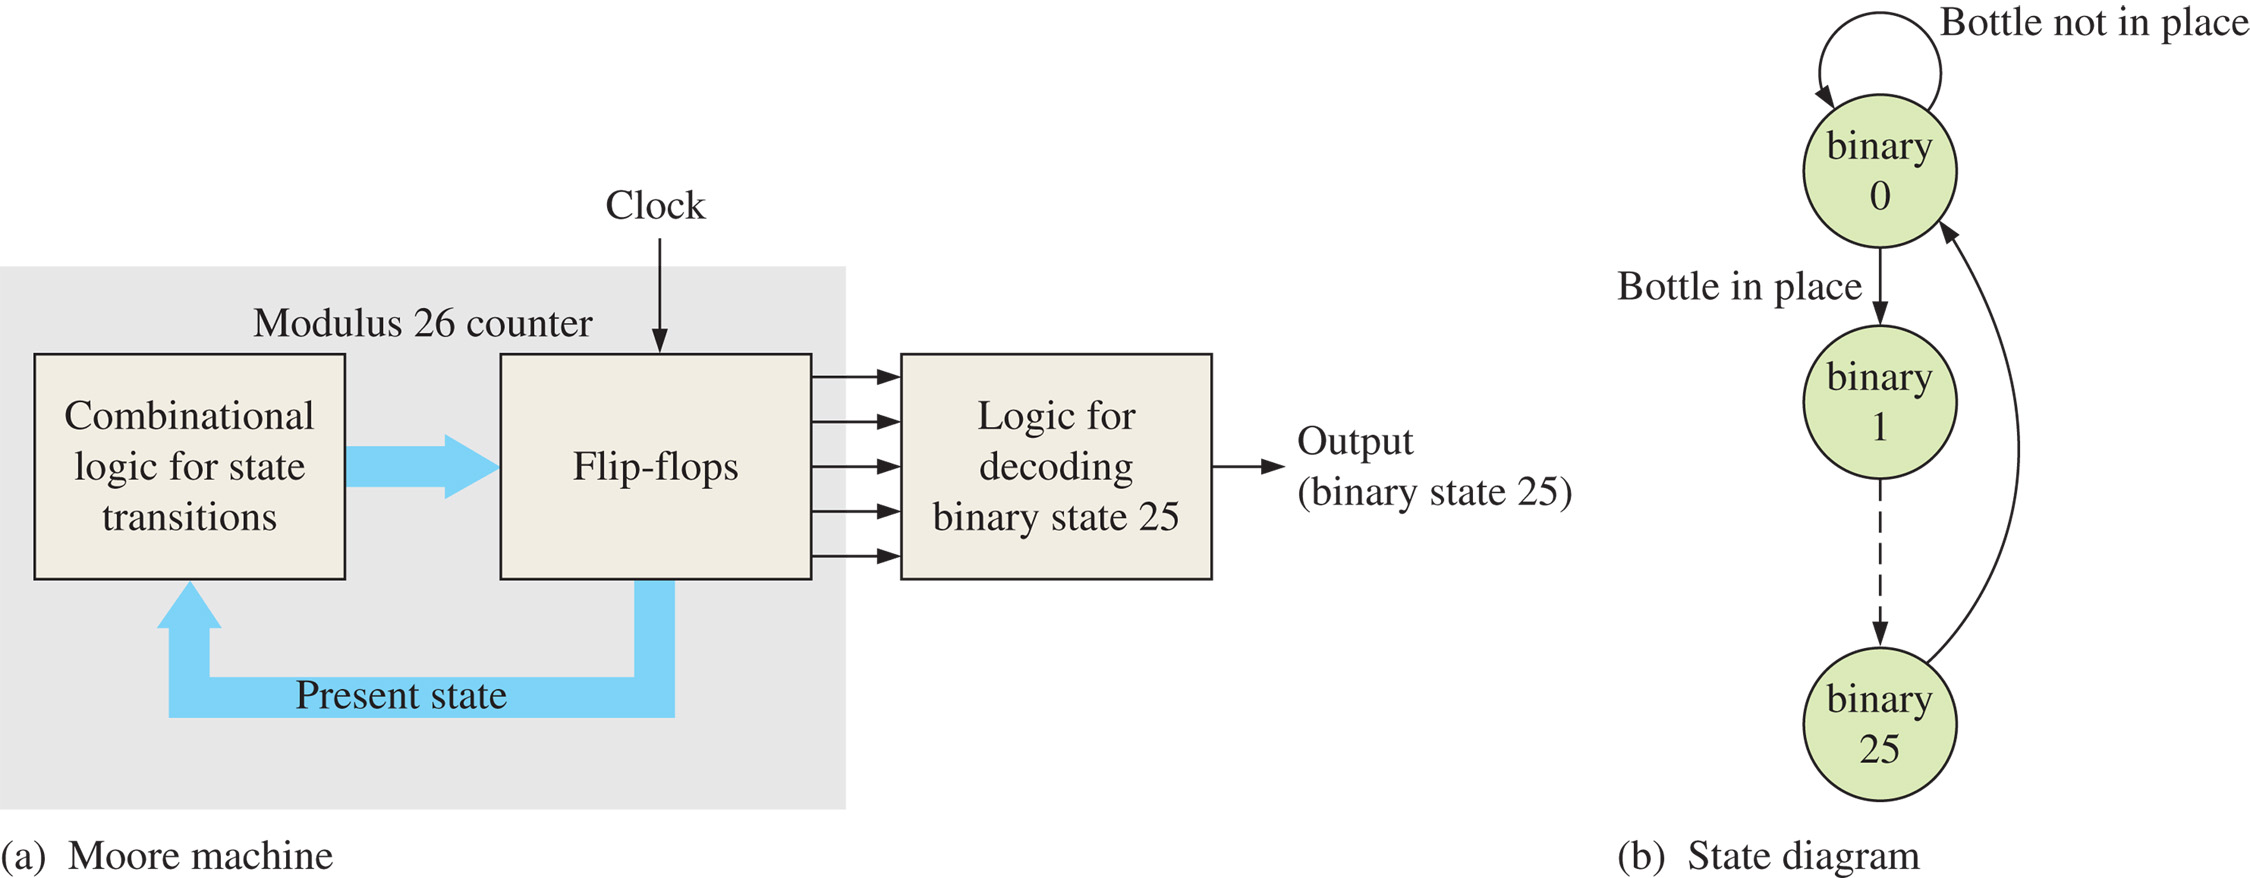
\includegraphics[width=0.85\textwidth]{figures/counter_3.jpg}
\caption{\small Example of a \textit{Moore machine}.}
\end{figure}
\end{frame}

\begin{frame}{Counters: Finite State Machines}
\begin{figure}
\centering
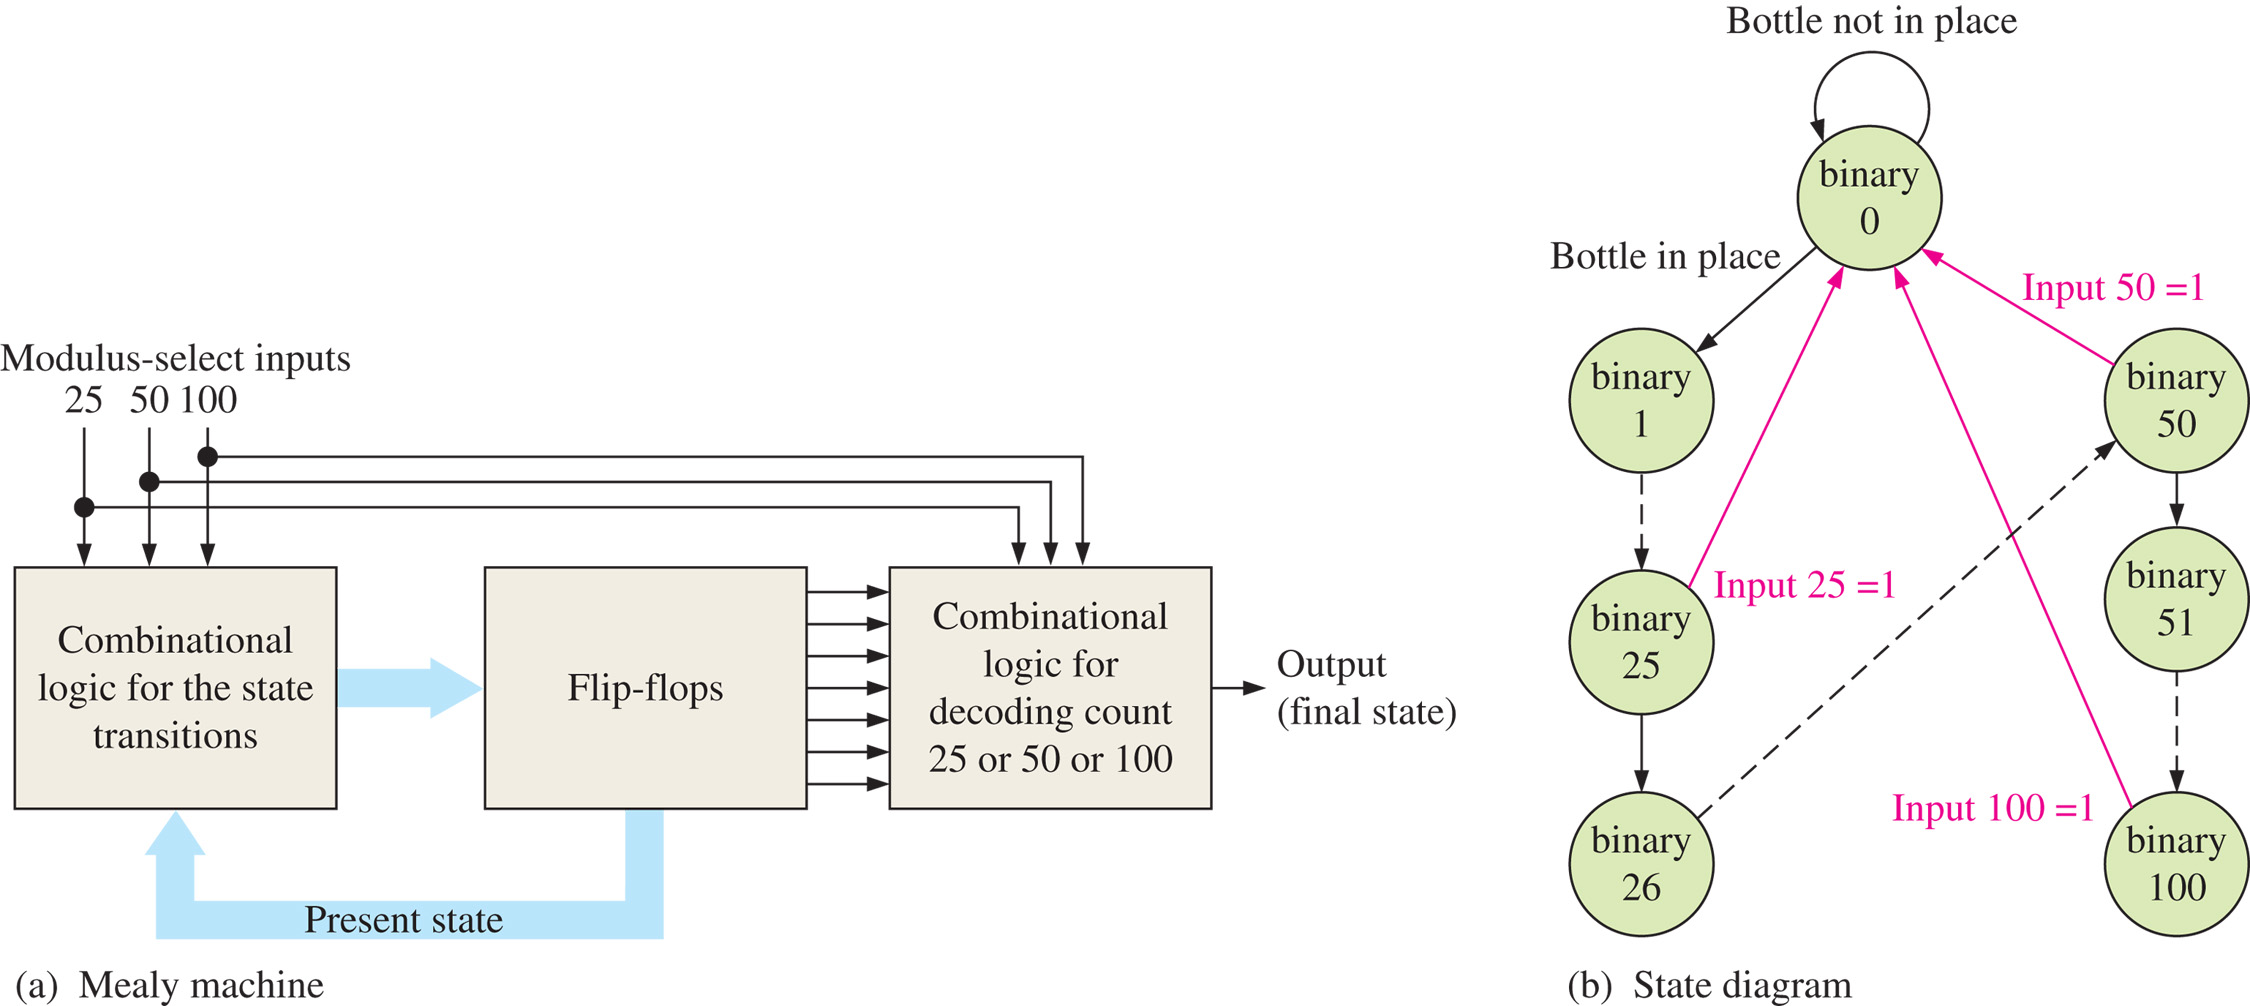
\includegraphics[width=0.85\textwidth]{figures/counter_4.jpg}
\caption{\small Example of a \textit{Mealy machine}.}
\end{figure}
\end{frame}

\begin{frame}{Counters: Asynchronous counters}
\begin{figure}
\centering
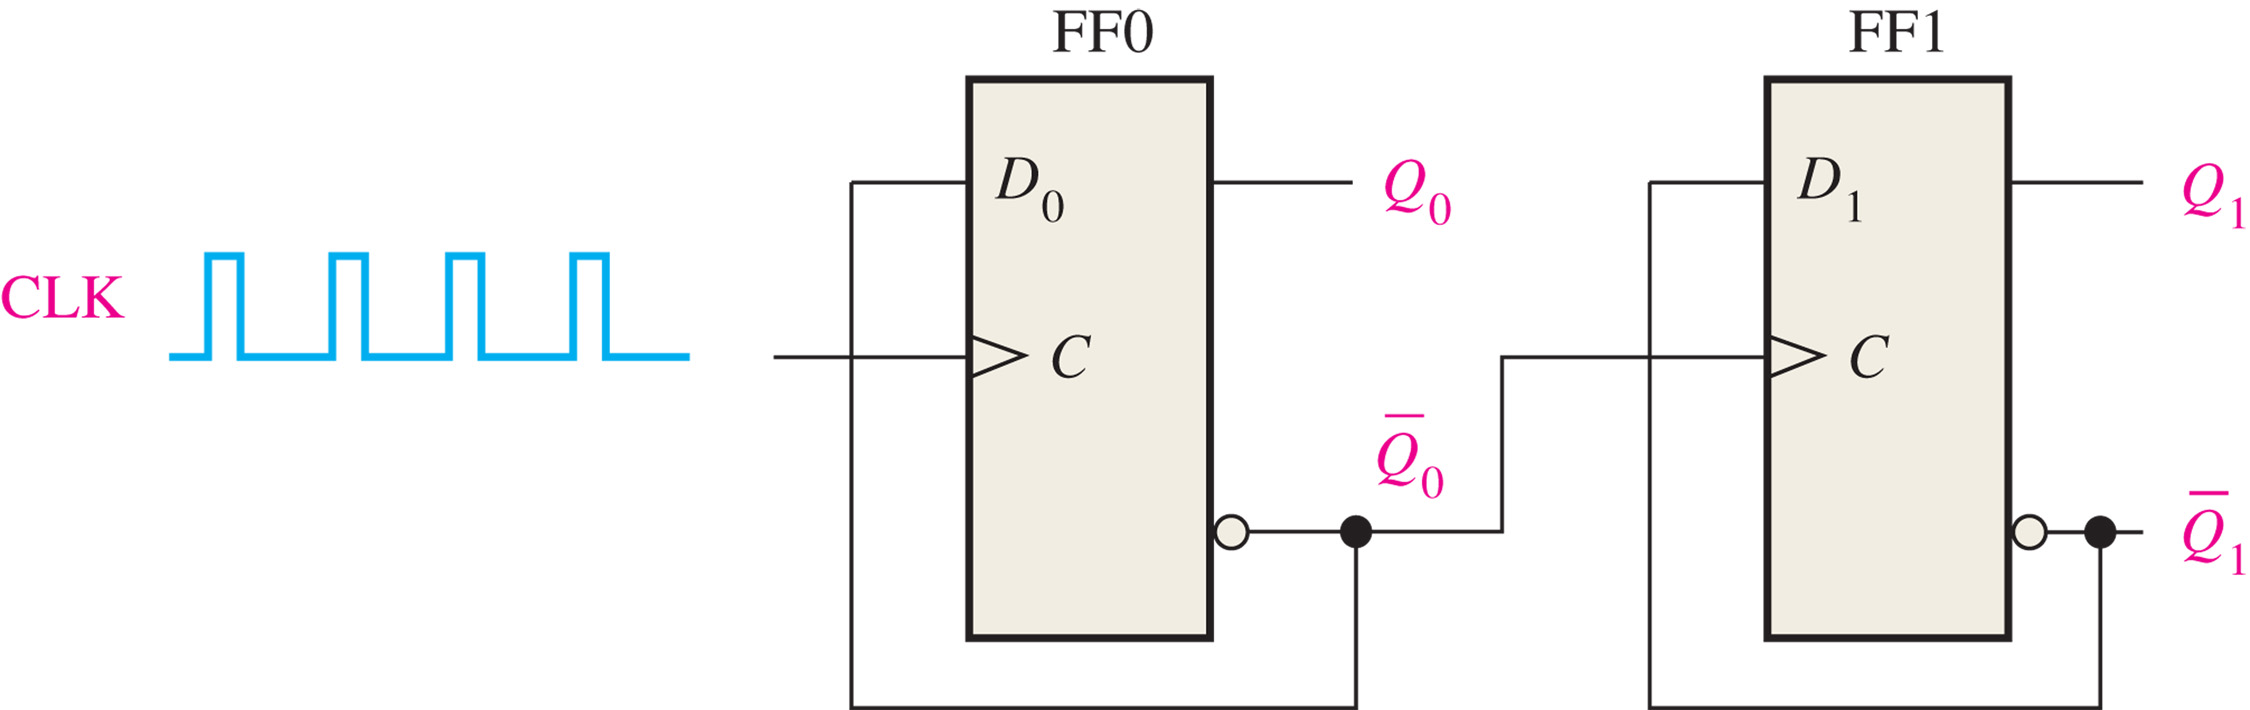
\includegraphics[width=0.65\textwidth]{figures/counter_5.jpg} \\ \vspace{0.5cm}
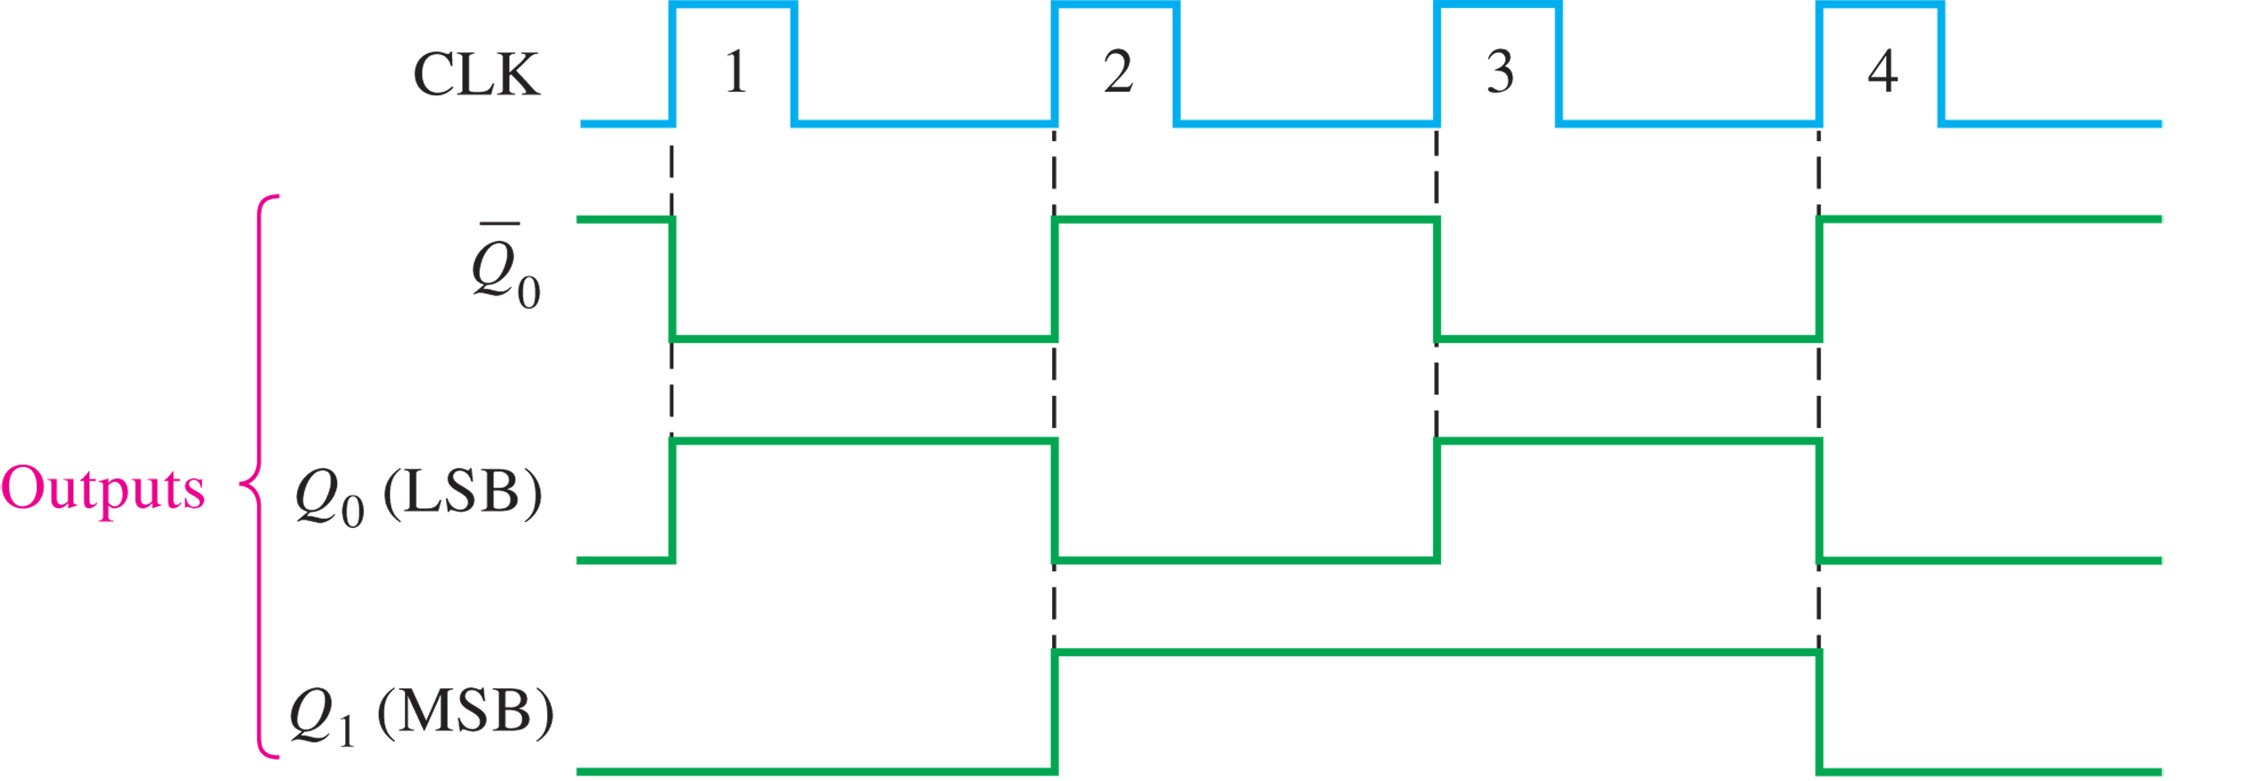
\includegraphics[width=0.65\textwidth]{figures/counter_6.jpg}
\caption{\small (Top) 2-bit asynchronous counter circuit diagram. (Bottom) Corresponding timing diagram.}
\end{figure}
\end{frame}

\begin{frame}{Counters: Synchronous counters}
\begin{figure}
\centering
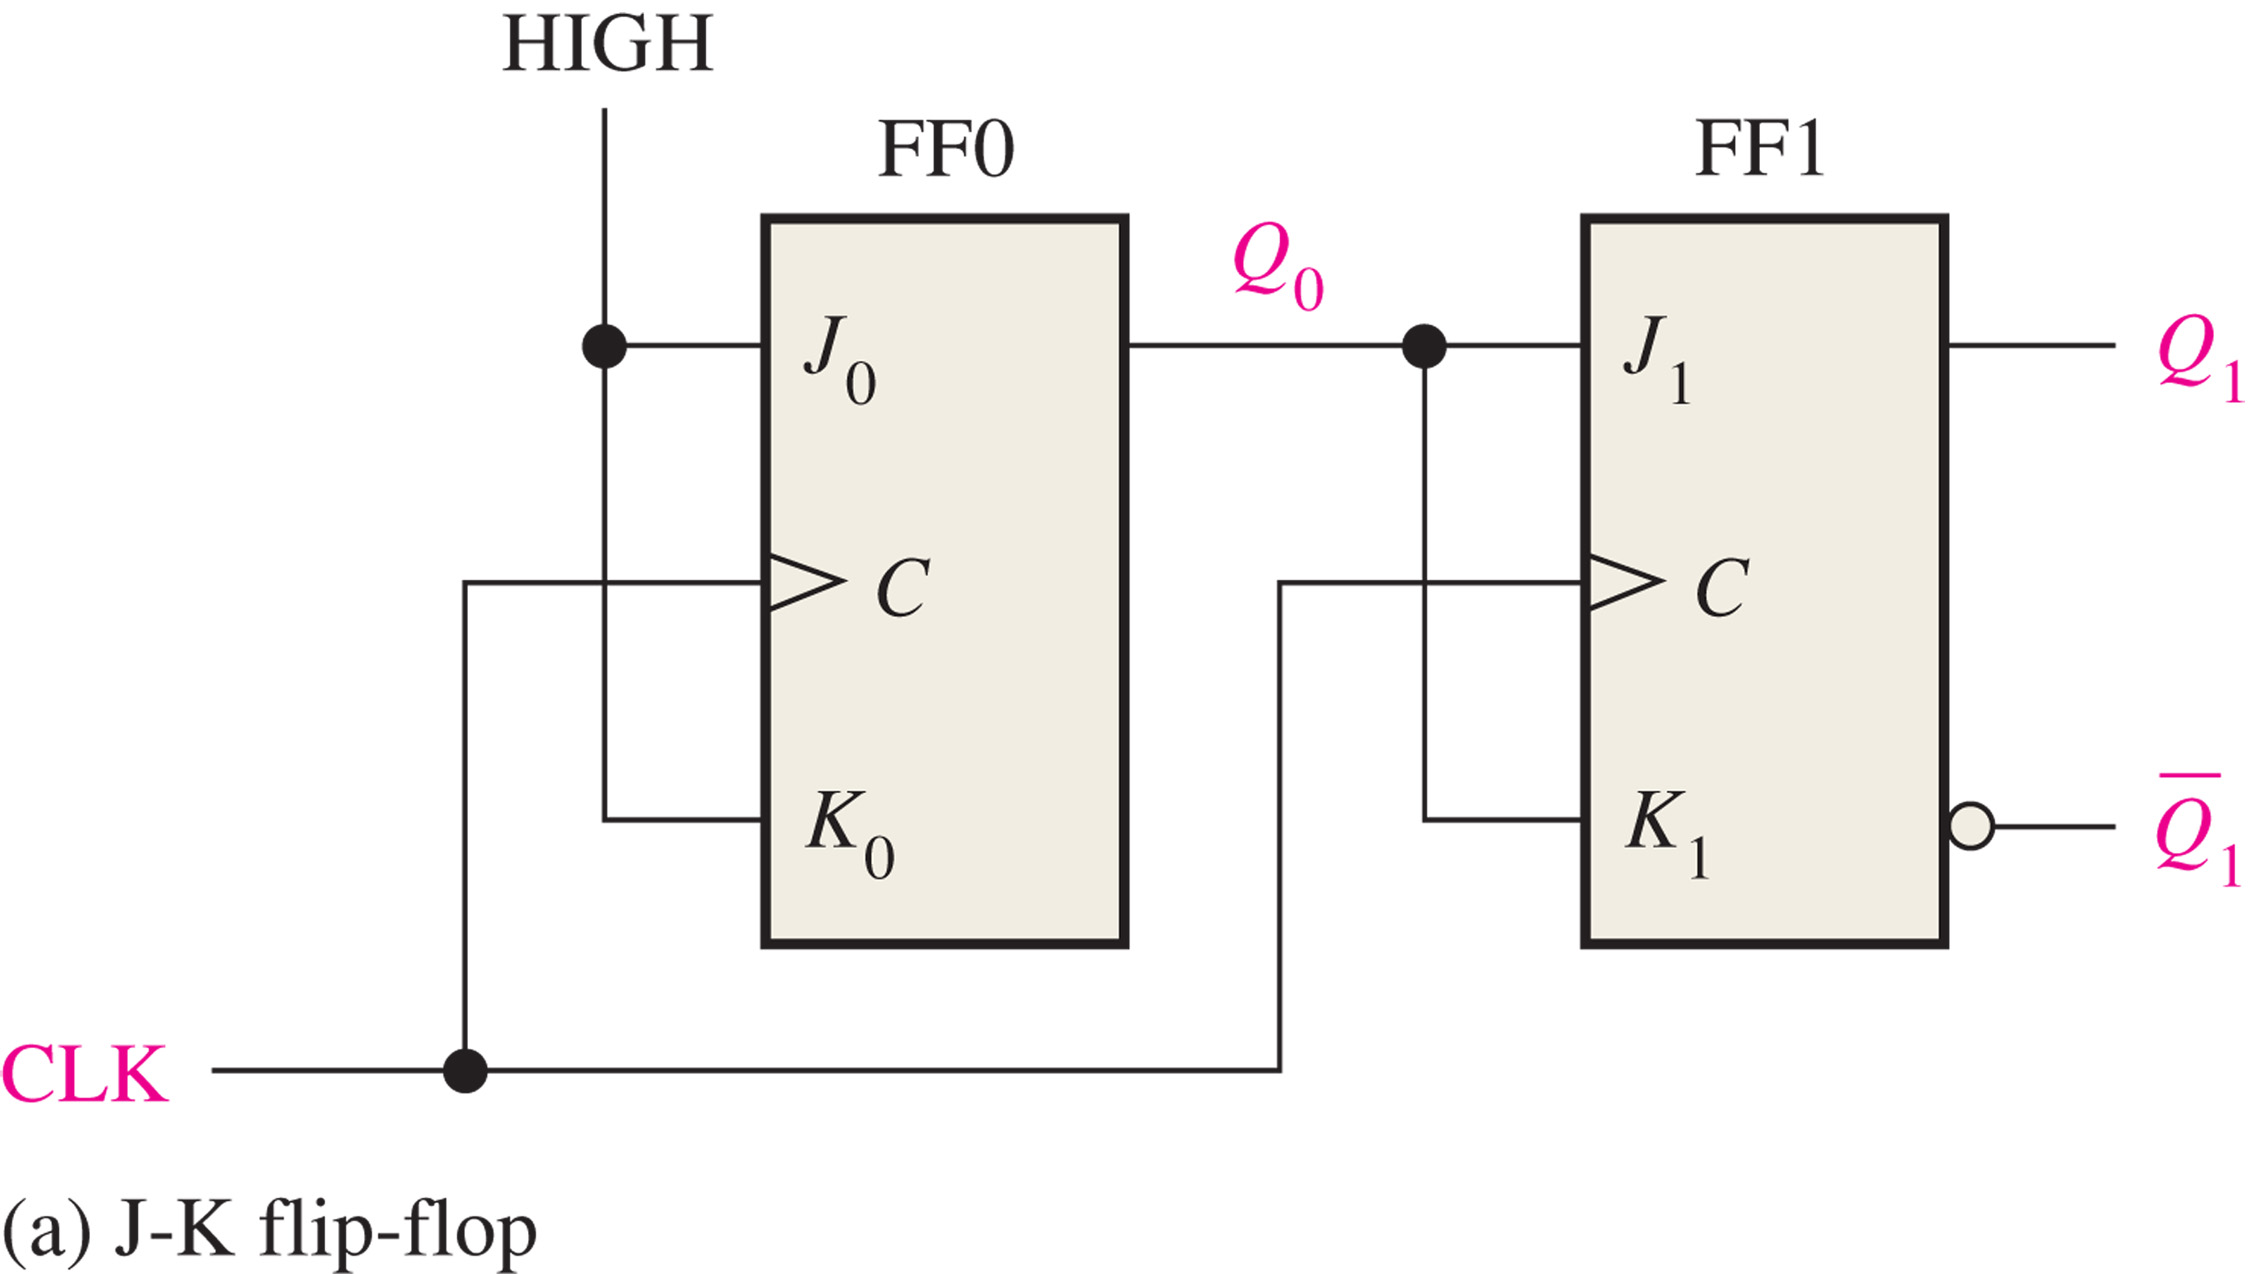
\includegraphics[width=0.5\textwidth]{figures/counter_7.jpg} \\ \vspace{0.5cm}
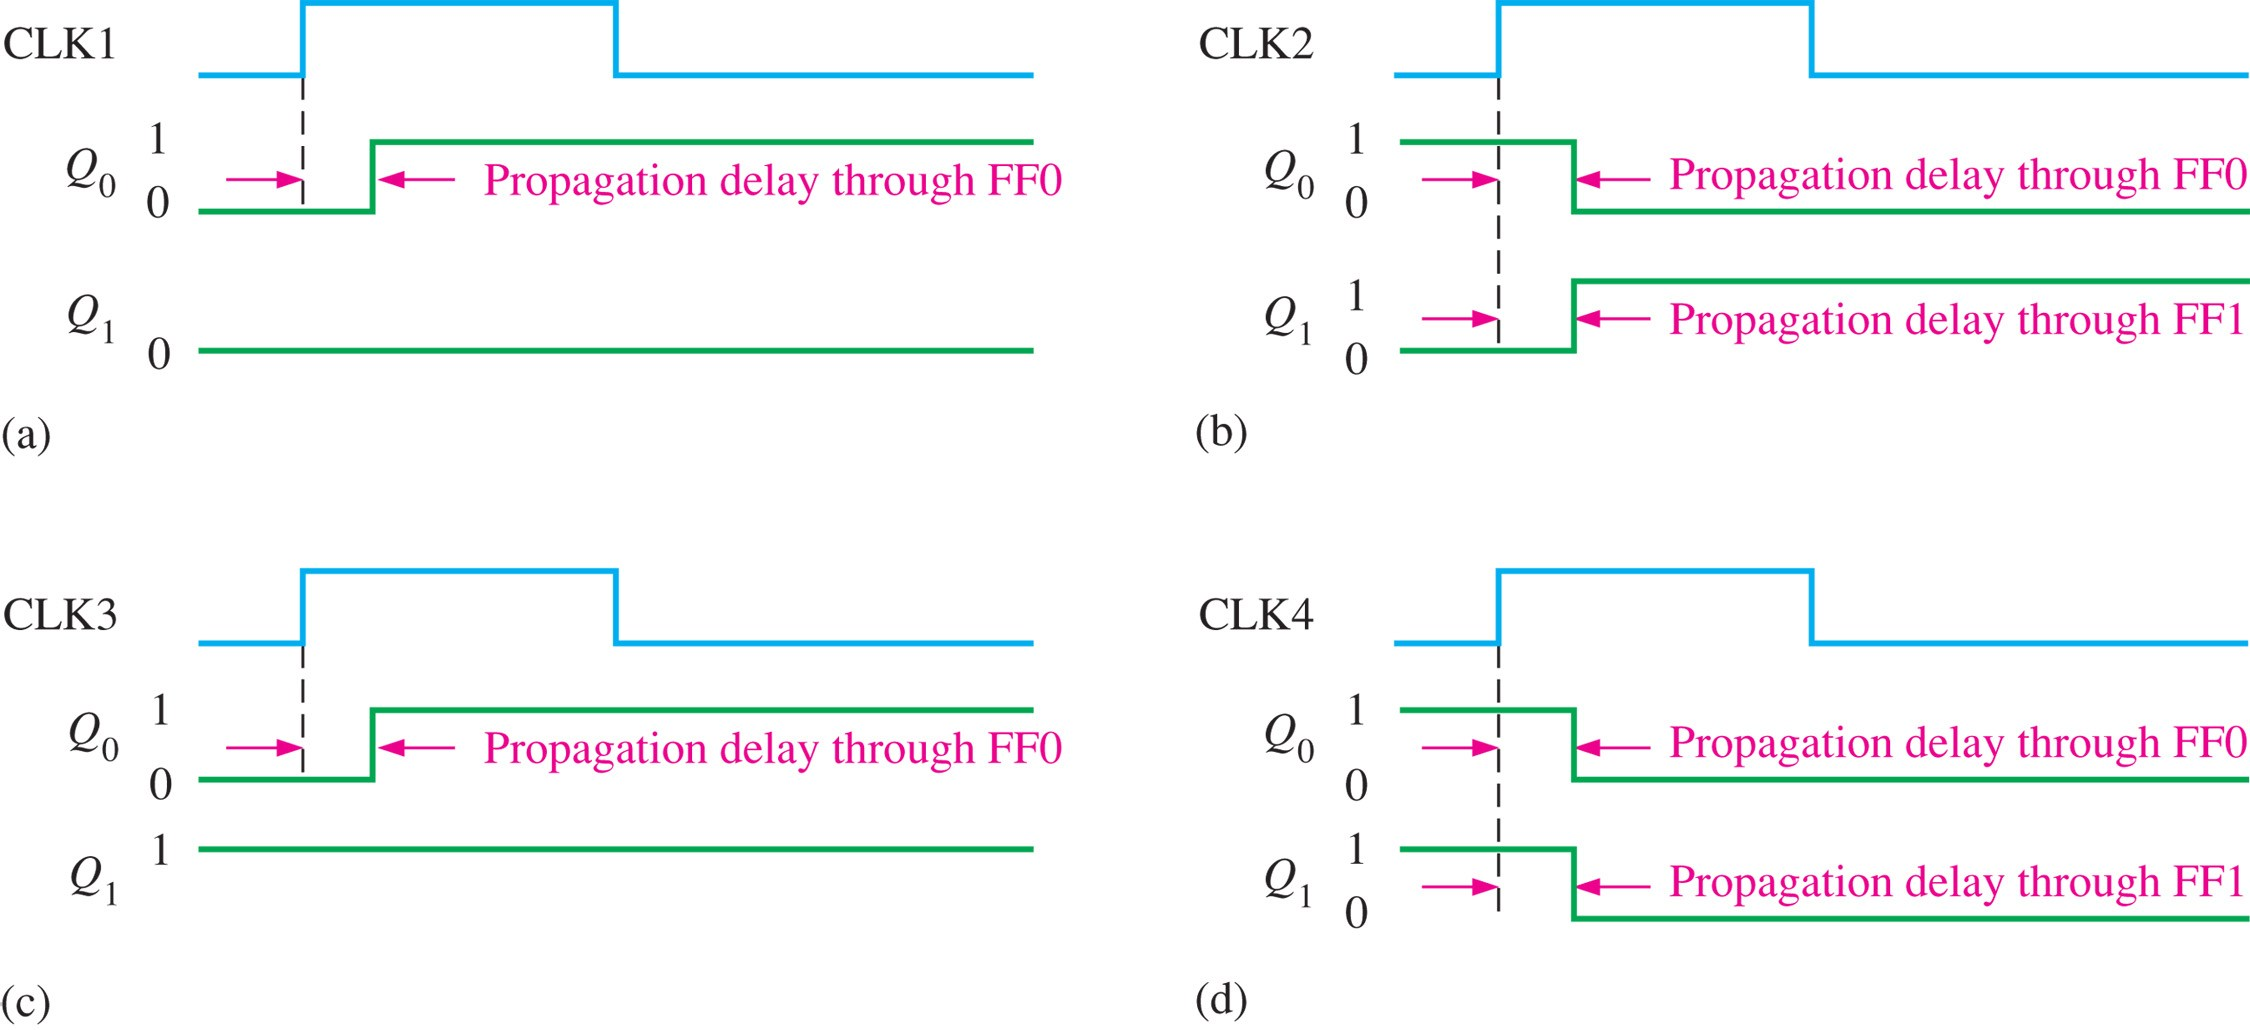
\includegraphics[width=0.5\textwidth]{figures/counter_8.jpg}
\caption{\small (Top) A 2-bit synchronous counter based on J-K flip flops.  (Bottom) Timing detail for the 2-bit synchronous counter.}
\end{figure}
\end{frame}

\begin{frame}{Counters: Synchronous counters}
\begin{figure}
\centering
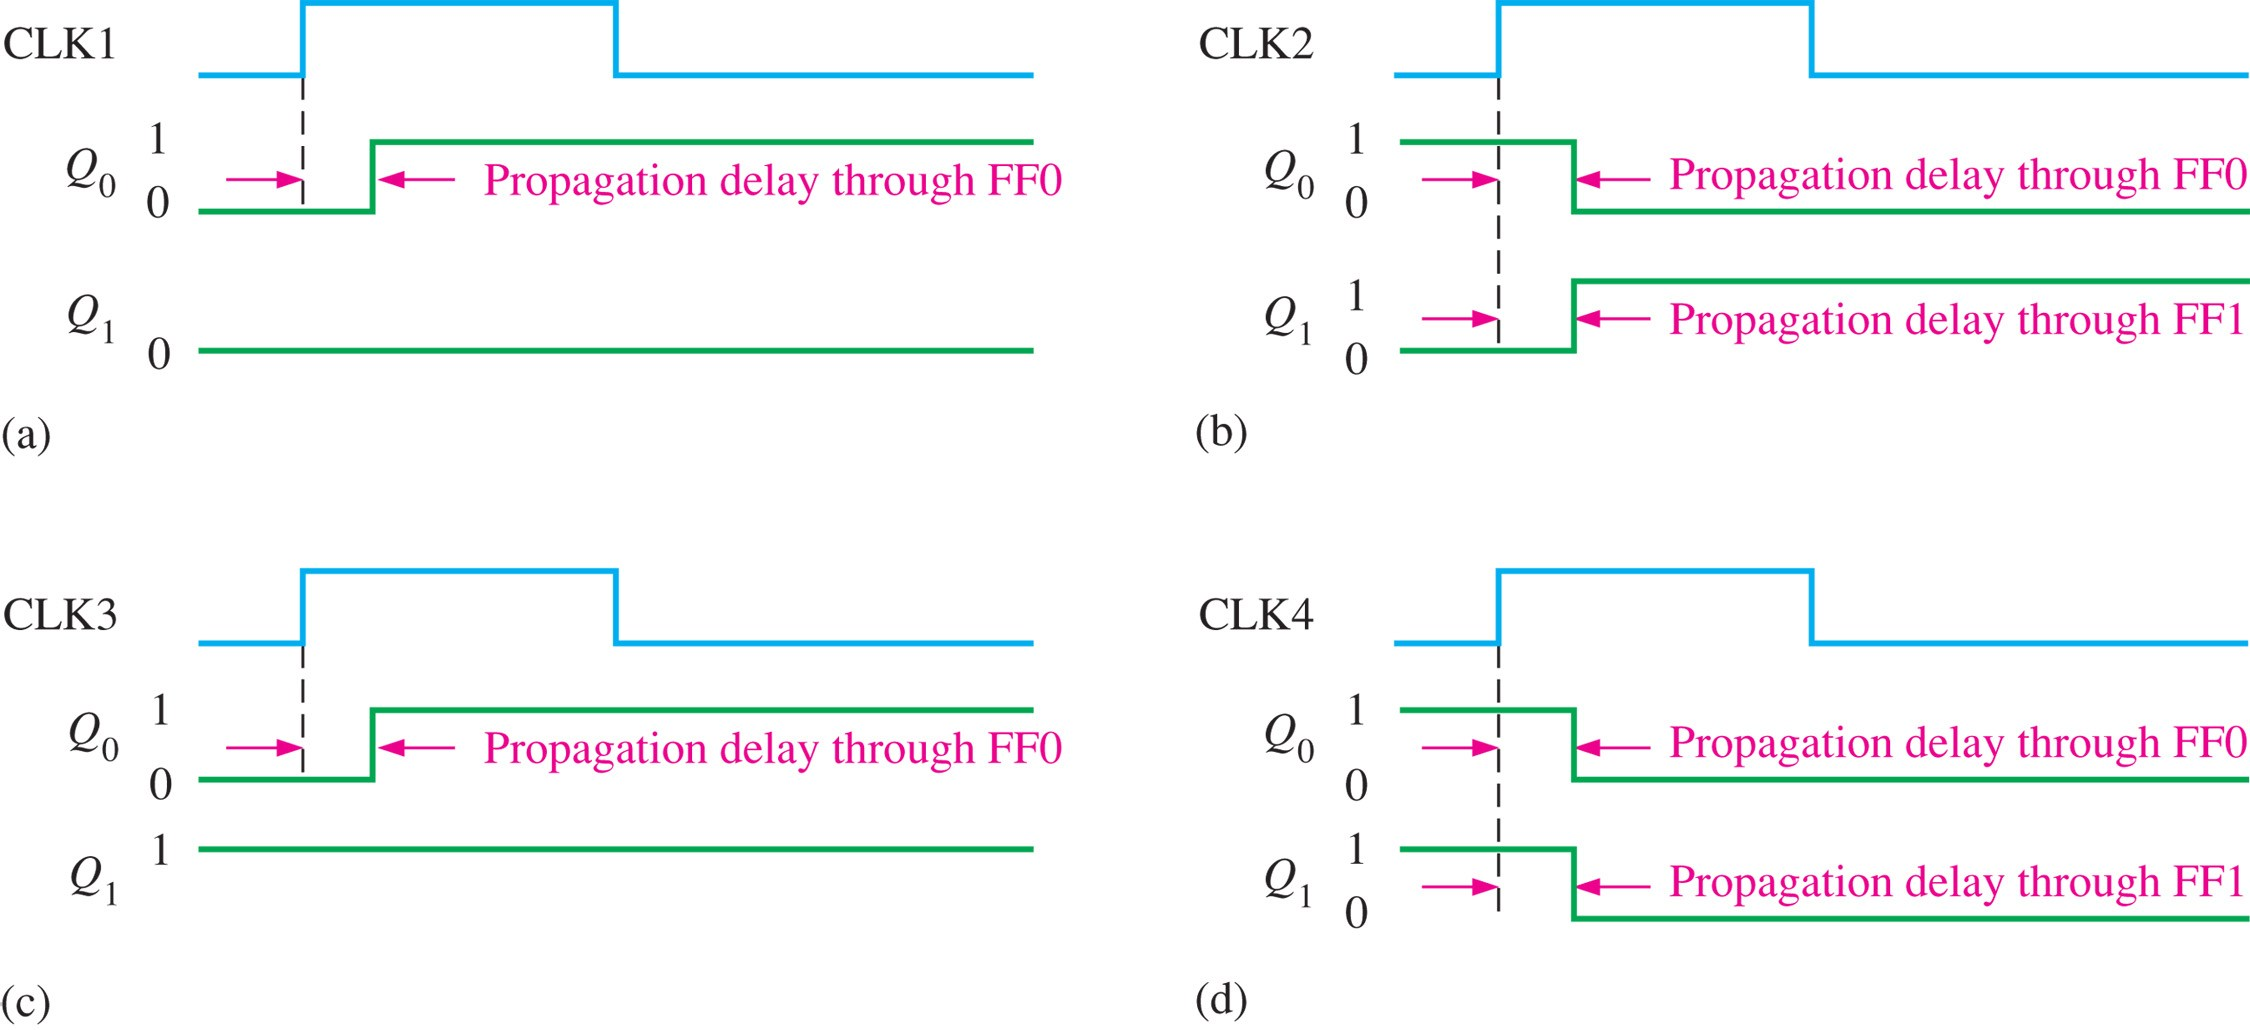
\includegraphics[width=0.5\textwidth]{figures/counter_8.jpg} \\ \vspace{0.5cm}
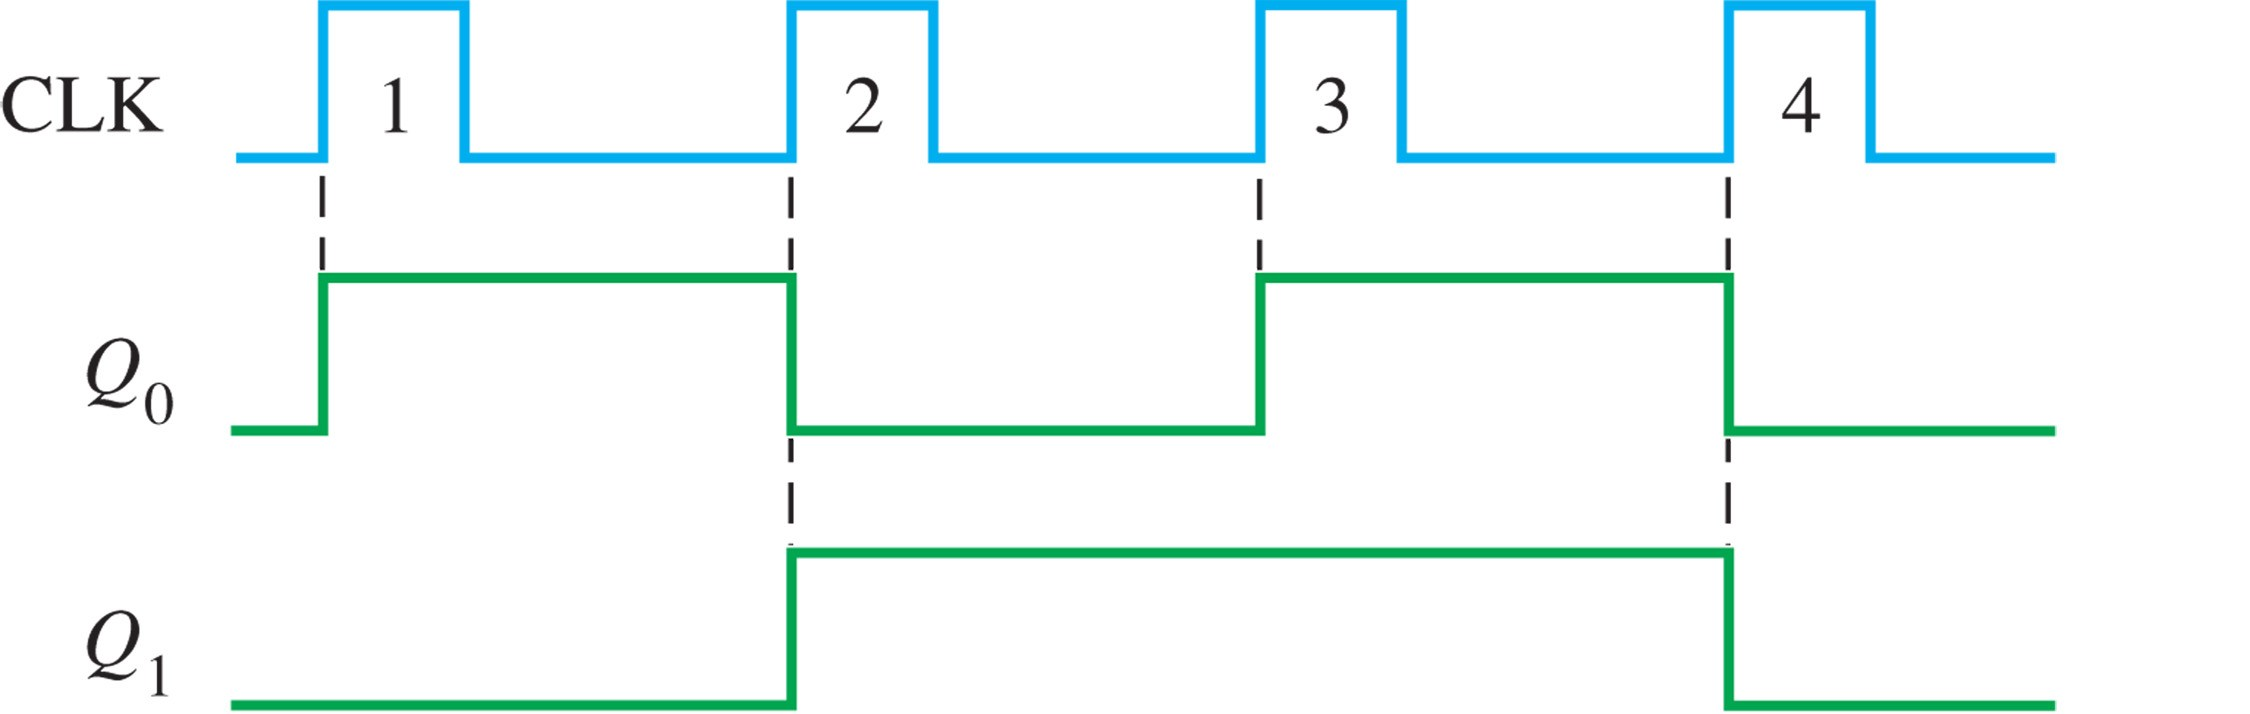
\includegraphics[width=0.5\textwidth]{figures/counter_9.jpg}
\caption{\small (Top) Timing detail for the 2-bit synchronous counter.  (Bottom) Full timing diagram.}
\end{figure}
\end{frame}

\begin{frame}{Counters: Synchronous counters}
\begin{figure}
\centering
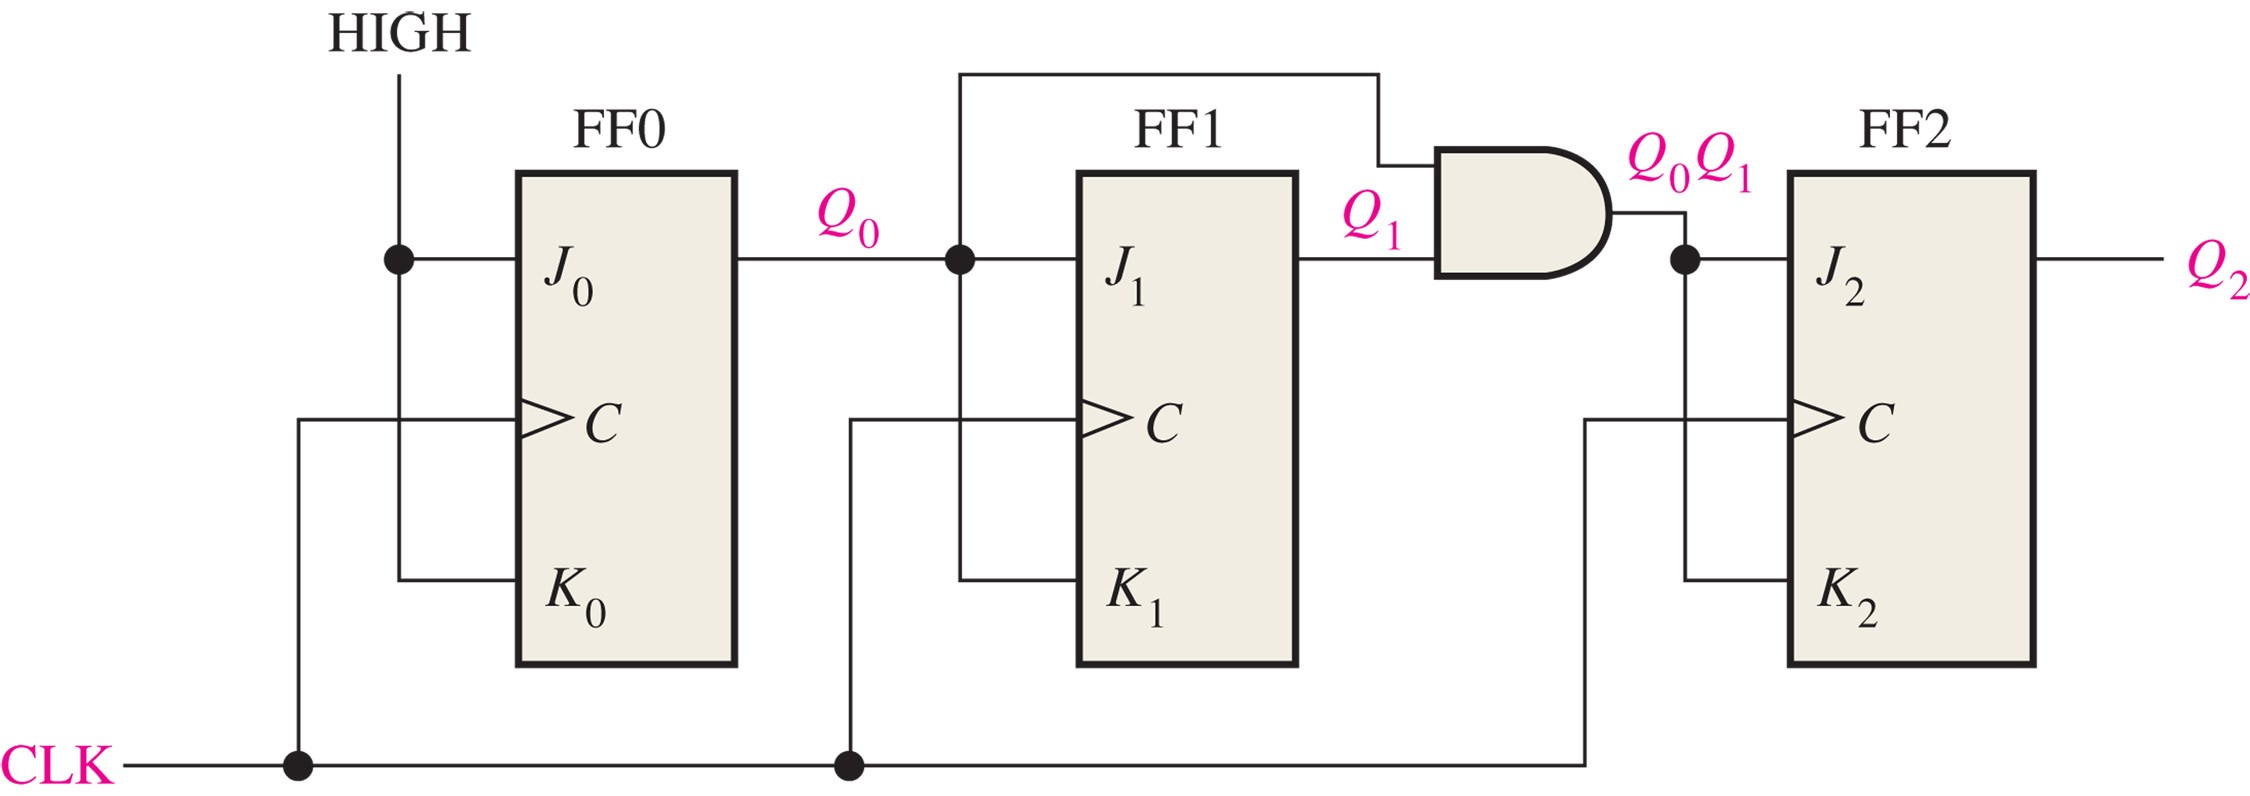
\includegraphics[width=0.85\textwidth]{figures/counter_10.jpg}
\caption{\small A 3-bit synchronous counter requires a steering gate.}
\end{figure}
\end{frame}

\begin{frame}{Counters: Synchronous counters}
\begin{figure}
\centering
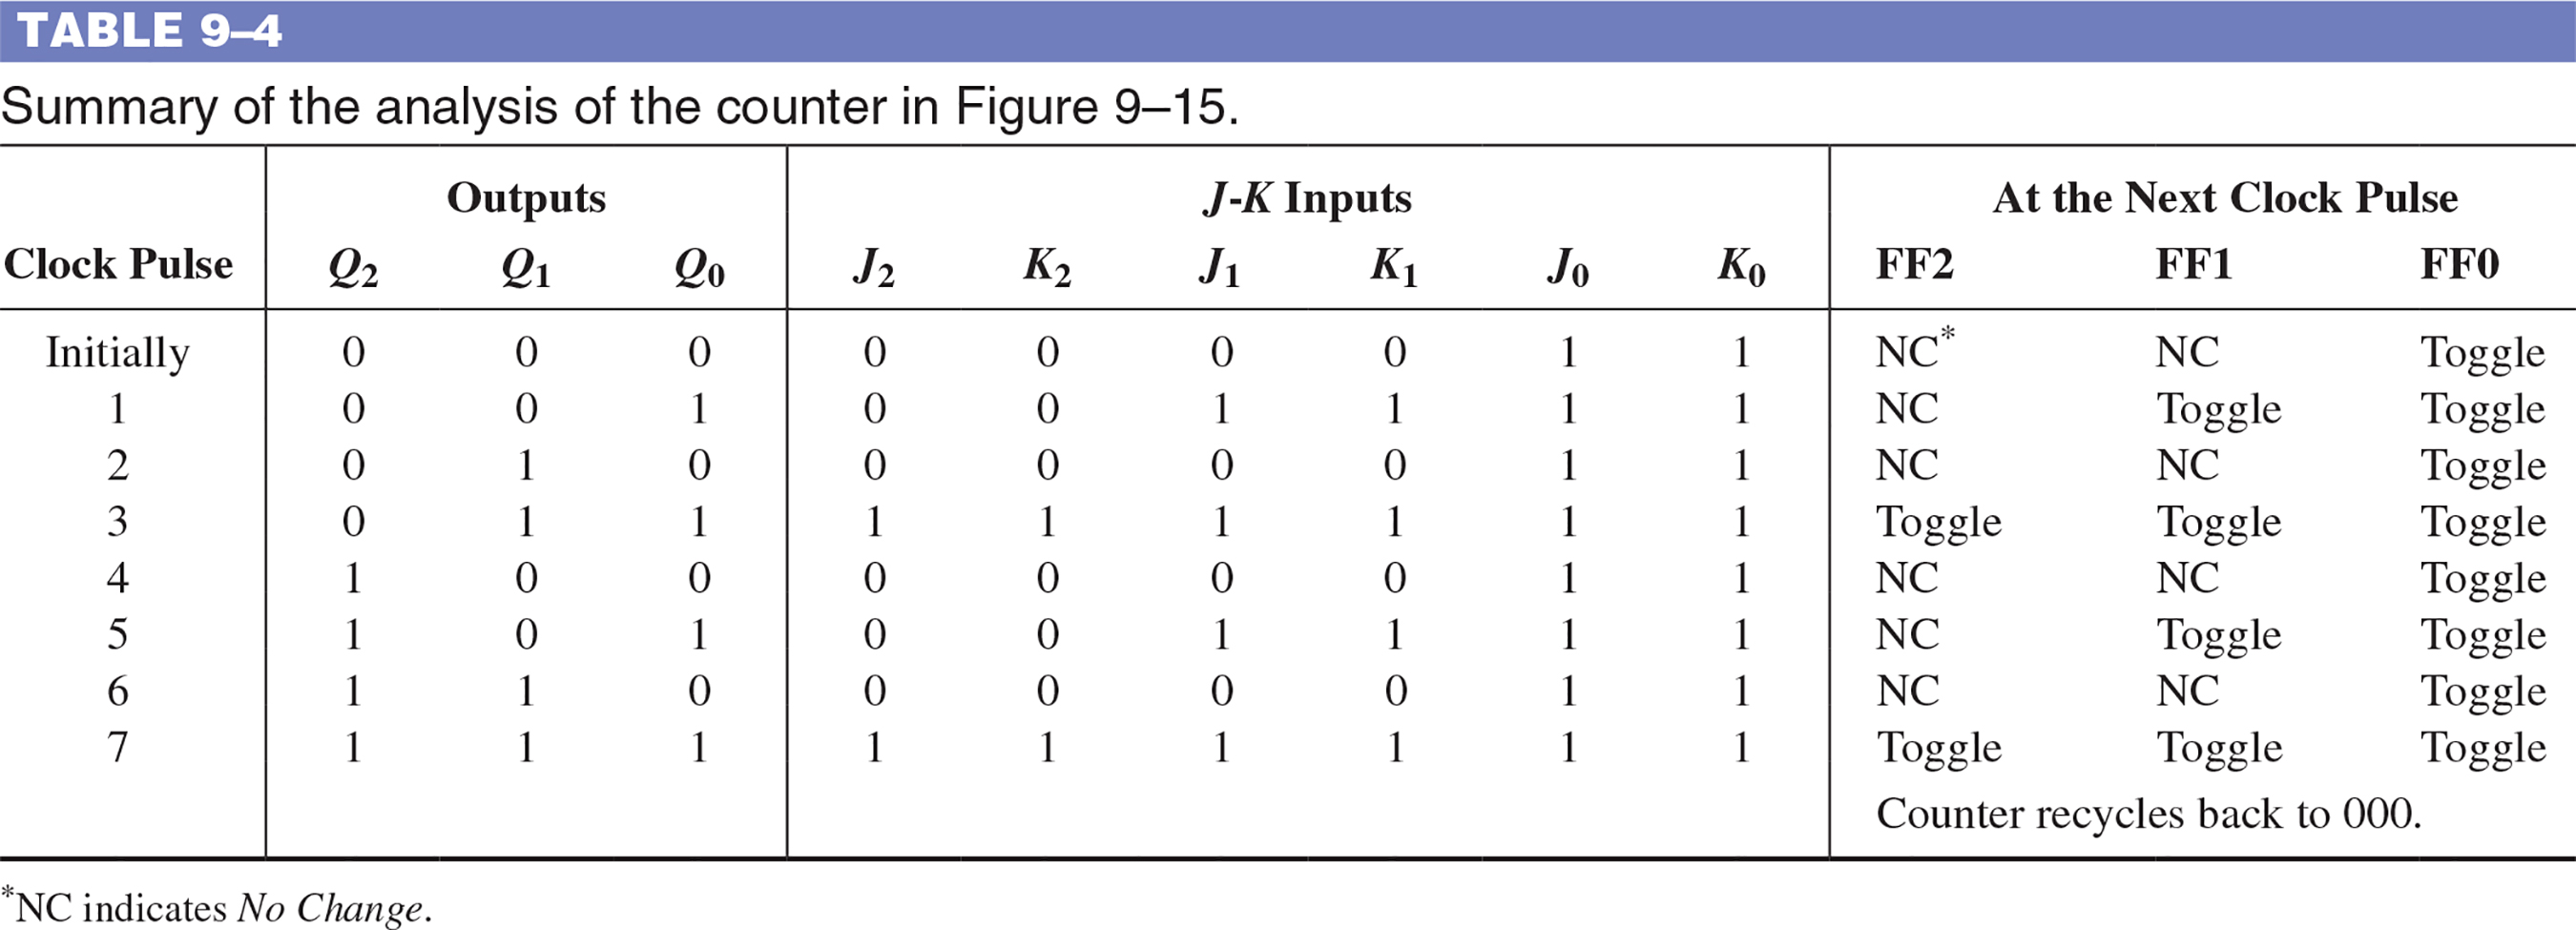
\includegraphics[width=0.9\textwidth]{figures/counter_13.jpg}
\caption{\small The internal states, and outputs for a 3-bit synchronous counter from J-K flip-flops.}
\end{figure}
\end{frame}

\section{Conclusion}

\begin{frame}{Unit 3 Summary}
\alert{Reading: chapter 8, 9} \\
\begin{enumerate}
\item Shift-Registers
\begin{itemize}
\item Shift register I/O
\item Load, shift, and bidirectional functions
\item Shift register counters
\item Application examples
\end{itemize}
\item Counters
\begin{itemize}
\item Finite State Machines (FSMs)
\item Asynchronous/Synchronous counters
\item Up/Down functions
\item Cascaded counters
\item Counter decoding
\item Counter Applications
\end{itemize}
\end{enumerate}
\end{frame}

\end{document}
